
\section{Breakup}
\newcommand{\zbx}{Z^{(b)}_x(\xi,\vecr_x)}
%\newcommand{\images}{images}
\newcommand{\bx}{\mathbf{x}}
\newcommand{\by}{\mathbf{y}}
%-------------------------------

%-----------------------------
\subsection{The CDCC method}

\slide{}
\begin{center}
\psframebox[fillcolor=green!10,linecolor=blue,framearc=0.1,fillstyle=solid,framesep=5pt]{
Inclusion of breakup channels: the CDCC method
}%psframe
\end{center} 
\end{frame}




%------------------------------------
\slide{Breakup modelspace}

\begin{figure}{\par \resizebox*{0.2\textwidth}{!}
{\includegraphics{\images/be10d_modelspace_bu.eps}} \par}
\end{figure}

\vspace{1cm}

\begin{center}
\psframebox[fillcolor=yellow!40,fillstyle=solid,framearc=0.2]{
\parbox{0.8\columnwidth}{%
\ding{43}{\em \small We want to include explicitly in the modelspace the breakup channels of the projectile or target.}
}%parbox
}%psframe
\end{center}

%\ding{43} In a transfer calculation, the modelspace will contain states belonging to different mass partitions.


\end{frame}



% ----------------------------------------------------------------------------------------------------
\slide{The CC method for bound states}
We need to incorporate explicitly in the Hamiltonian the internal structure of the nucleus being excited (eg.~ {\verde target}).
$$ 
\psframebox[linecolor=red,framearc=0.1]{
 H = T_R   +  h(\xi)+ V(\bR, \xi)
}
$$


\begin{itemize}
\gitem{$T_R$}: Kinetic energy for projectile-target relative motion.
\gitem{$\{\xi\}$}: Internal degrees of freedom of the target (depend on the model).
\gitem{$h(\xi)$}: Internal Hamiltonian of the target.
$$
\psframebox[linecolor=red,framearc=0.1]{
h(\xi)\phi_{n}(\xi)  =  \varepsilon_{n}\phi_{n}(\xi)
}
$$

\gitem{$V(\bR, \xi)$}: Projectile-target interaction %, eg:
% $$ V(\bR, \xi) = \sum_{i=1}^{N} V_{pi}(\br_{pi}) $$

% \pause 
% \item[] {\bf Eg.:} $^7$Li=$\alpha+t$ $\Rightarrow$ {\verde $\{\xi\} \equiv \bf r$}
% $$
% V_\mathrm{p-7Li}({\bf R}, {\bf r})= V_\mathrm{p-t}\left({\bf R} +\frac{4}{7}{\bf r}\right) 
% + 
% V_\mathrm{p-\alpha}\left({\bf R} +\frac{3}{7}{\bf r}\right)
% $$
\end{itemize}
\end{frame}





% ----------------------------------------------------------------------------------------------------
\slide{The CC method (continued): CC model wavefunction}

We expand the total wave function in a subset of internal states (the {\cal P} space):
$$
\psframebox[linecolor=red,framearc=0.1]{
\Psi^{(+)}_\mathrm{model}(\bR,\xi)=\phi_{0}(\xi)\chi_{0}(\bR)+ \sum_{n>0} \phi_{n}(\xi)\chi_{n}(\bR)  
}
$$

Boundary conditions for  the $\chi_{n}(\bR)$ (unknowns):

\begin{align*}
\chi_0^{(+)}(\bR) & \rightarrow  e^{i \bK_0 \cdot \bR}  + {\red f_{0,0}(\theta)} \frac{e^{i K_0 R}}{R} 
\quad \quad  \textrm{\blue for n=0 (elastic)} \\
\chi_n^{(+)}(\bR) & \rightarrow                           {\red f_{n,0}(\theta)} \frac{e^{i K_n R}}{R} 
\quad  \quad \quad \quad \textrm{\blue for n>0 (non-elastic)}
\end{align*}

\end{frame}





% ----------------------------------------------------------------------------------------------------
\slide{The CC method (continued): calculation of $\chi_n^{(+)}(\bR)$; the coupled equations}

\begin{itemize}
\item The model wavefunction must satisfy the Schr\"odinger equation:
$$
 [H-E]\Psi^{(+)}_\mathrm{model}(\bR,\xi)=0
$$

\item Projecting onto the internal states one gets a system of coupled-equations for the functions 
{\verde $\{\chi_{n}(\bR) \}$:}
$$
\psframebox[linecolor=red,framearc=0.1]{
\left[E-\varepsilon_{n}-T_R -V_{n,n}(\bR) \right] \chi_{n}(\bR)  = 
\sum_{n' \neq n} V_{n,n'}(\bR) \chi_{n'}(\bR) 
}%psframebox
$$


\item The structure information is embedded in the {\verde coupling potentials:}
$$
\psframebox[linecolor=red,framearc=0.1]{
V_{n,n'}(\bR) = \int   d \xi \phi_{n'}(\xi)^* V(\bR, \xi) \phi_{n}(\xi) 
}%psframebox
$$

\item[\ding{43}] {\small \em \blue $\phi_{n}(\xi)$ will depend on the structure model 
(collective, single-particle,etc).}

\end{itemize}
\end{frame}



% -------------------------------------------------------------------------------------------------
\slide{Choice of structure model: the few-body (cluster) case}


\bc
\column{0.45\linewidth}
\begin{center}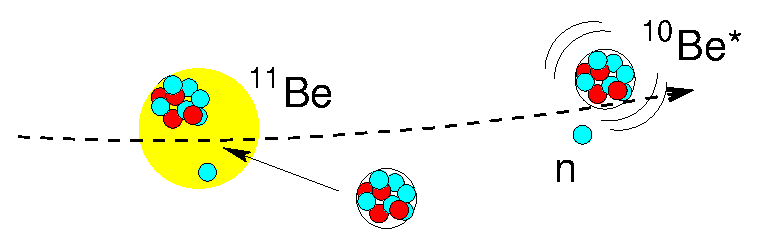
\includegraphics[width=0.85\columnwidth]{\images/be11t_mic.eps}\end{center}
\begin{center} $${\cal V}_{pt} = \sum_{ij} V_{ij}(\br_{ij})$$  \end{center}

\column{0.15\linewidth}
\begin{center}\includegraphics[width=0.7\columnwidth]{\images/arrow-blue.eps}\end{center}
\column{0.45\linewidth}
\begin{center}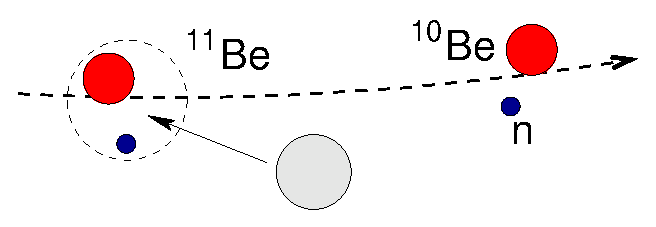
\includegraphics[width=0.85\columnwidth]{\images/be11t_inert.eps}\end{center}
\begin{center}$${\cal V}_{pt} = U_{ct}(\br_{ct}) + U_{nt}(\br_{nt})$$\end{center}

\ec

\bi

\bigskip

\item Effective {\blue three-body} Hamiltonian:
$$
\psframebox[linecolor=red,fillcolor=orange!10,fillstyle=solid,framearc=0.2]{
H = T_\bR   +  h_r(\br) + U_{ct}(\br_{ct}) + U_{nt}(\br_{nt})
}%psframe
$$ 


\item $U_{ct}(\br_{ct})$, $U_{nt}(\br_{nt})$ are optical potentials describing fragment-target elastic scattering (eg.~target excitation is treated effectively, through absorption) 


\ei

\end{frame}


% ----------------------------------------------------------------------------------
\slide{Inelastic scattering in a few-body model}

\begin{itemize}
\gitem{Some nuclei allow a description in terms of two or more clusters:} \\ 
d=p+n,  \nuc{6}{Li}=$\alpha$+d, \nuc{7}{Li}=$\alpha$+\nuc{3}{H}. 

\gitem{Projectile-target interaction:}
 $$ 
 V(\bR,\xi) \equiv V(\bR,\br)= U_{1}(\br_1) + U_2(\br_2)
 $$


\gitem{Transition potentials:}
 $$
\psframebox[linecolor=red,framearc=0.1]{
 V_{n,n'}(\mathbf{R})=\int d\mathbf{r}\phi_{n}^{*}(\br)\left[U_{1}(\br_1) + U_2(\br_2)\right] \phi_{n'}(\br)
}
$$ 

\pause 

%\parbox{0.7\textwidth}{
\psframebox[fillcolor=green!10,linecolor=blue,framearc=0.1,fillstyle=solid]{
\begin{minipage}{.55\textwidth}
%\begin{columns}
%\column{0.3\textwidth}
\textcolor{blue}{Example:} $^7$Li=$\alpha$+t
 $$
 \br_\alpha= \bR - \frac{m_t}{m_\alpha+m_t} \br ;
 \quad 
 \br_t= \bR + \frac{m_\alpha}{m_\alpha+m_t}\br
 $$
{\blue Internal states:} (two-body cluster model)
 $$[T_\br + V_{\alpha-t}(\br) - \varepsilon_n ]\phi_n(\br)=0$$
\end{minipage}
%\column{0.3\textwidth}
\begin{minipage}{.35\textwidth}
\begin{center}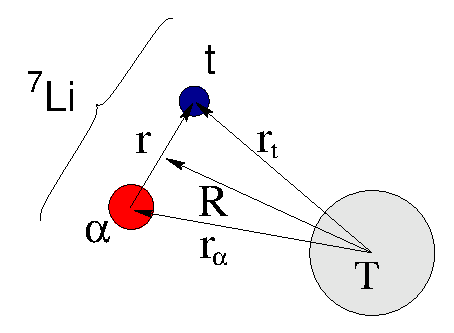
\includegraphics[width=0.7\columnwidth]{\images/li7t_coord.eps}\end{center}
%\end{columns}
\end{minipage}
%}%parbox
}%psframe


\end{itemize}

\end{frame}



% ----------------------------------------------------------------------------------
\slide{Example: \nuc{7}{Li}($\alpha$+$t$) +\nuc{208}{Pb} at 68 MeV}

%{\bf Example:} \nuc{7}{Li}($\alpha$+$t$) +\nuc{208}{Pb} at 68 MeV {\verde (Phys. Lett. 139B (1984) 150)}: 
%\ding{43}    Uses $\alpha$+t model for \nuc{7}{Li}
%$$
%V_{n,n'}(\bR)=\int d\br \phi_{n}^{*}(\br)
%\left[V_\mathrm{\alpha}(\br_{\alpha}) + V_\mathrm{t}(\br_{t}) \right]
%\phi_{n'}(\br)  ; \quad  n=0,1
%$$

\ding{233} CC calculation with 2 channels (3/2$^-$, 1/2$^-$)  {\verde (Phys. Lett. 139B (1984) 150)}
\begin{columns}
\column{0.4\textwidth}
\begin{center}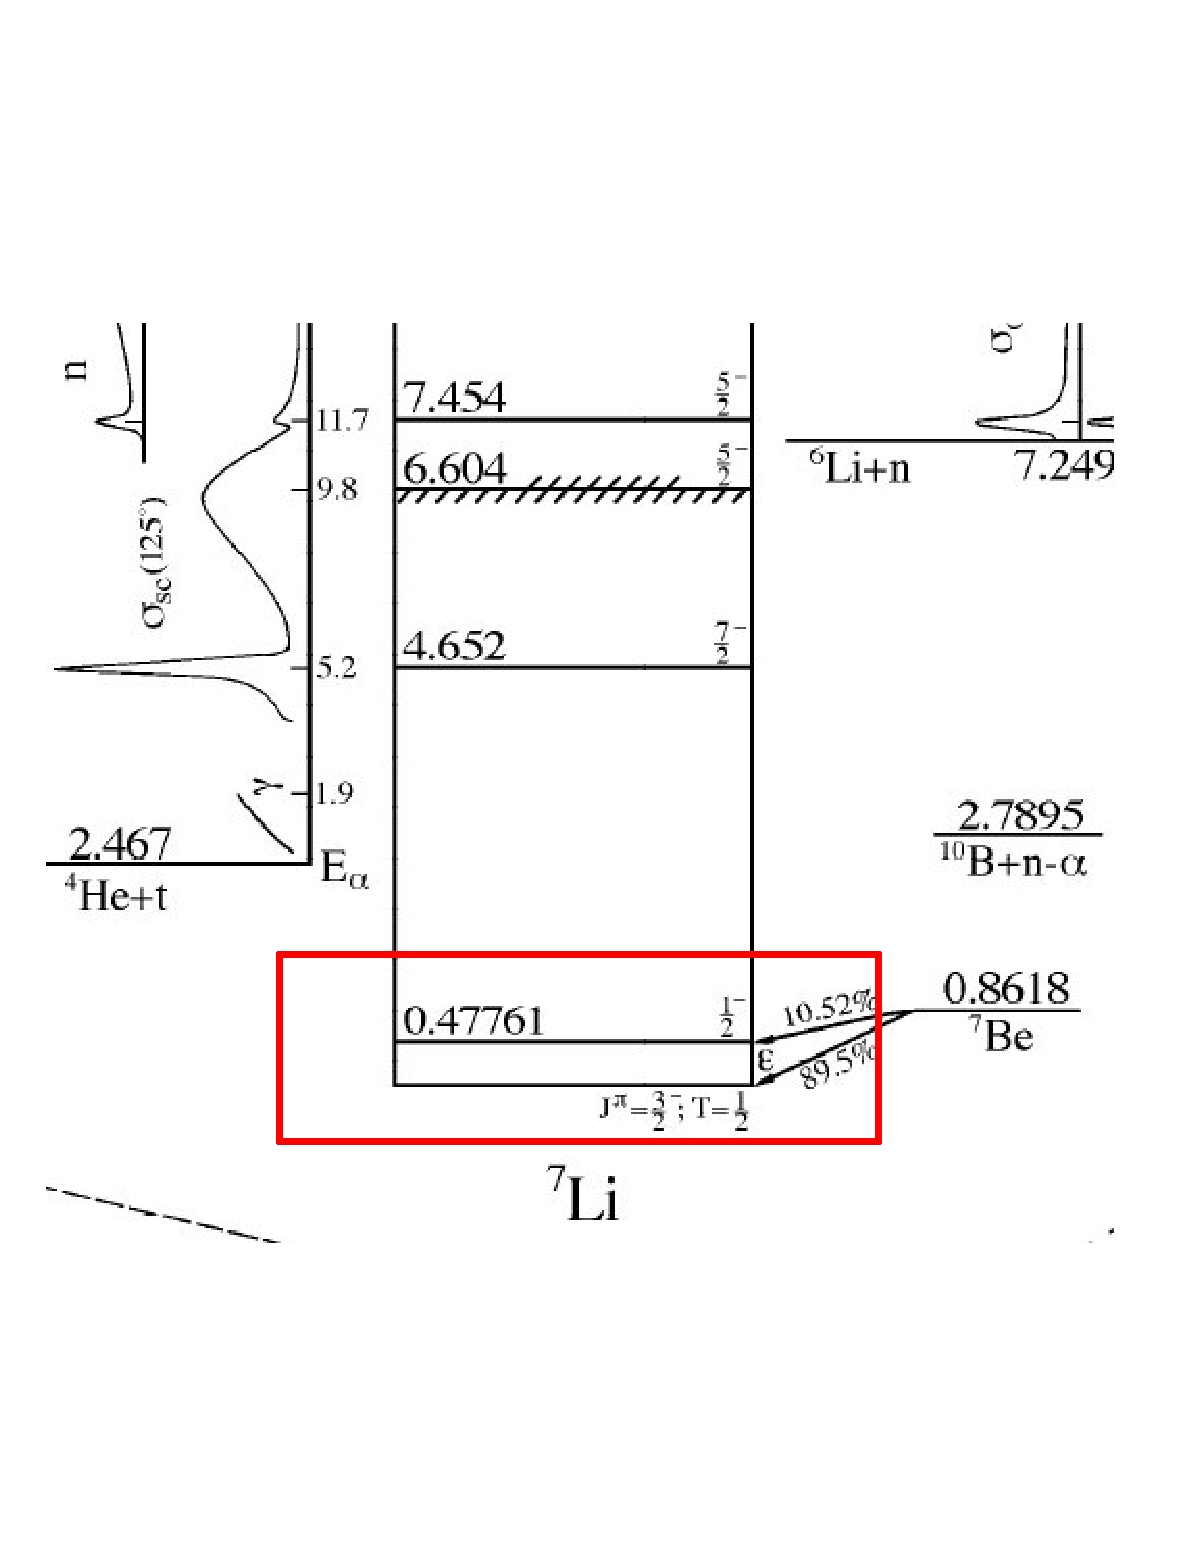
\includegraphics[height=6.0cm]{\images/li7spectrum2.eps} \end{center}
\column{0.5\textwidth}
\begin{center}
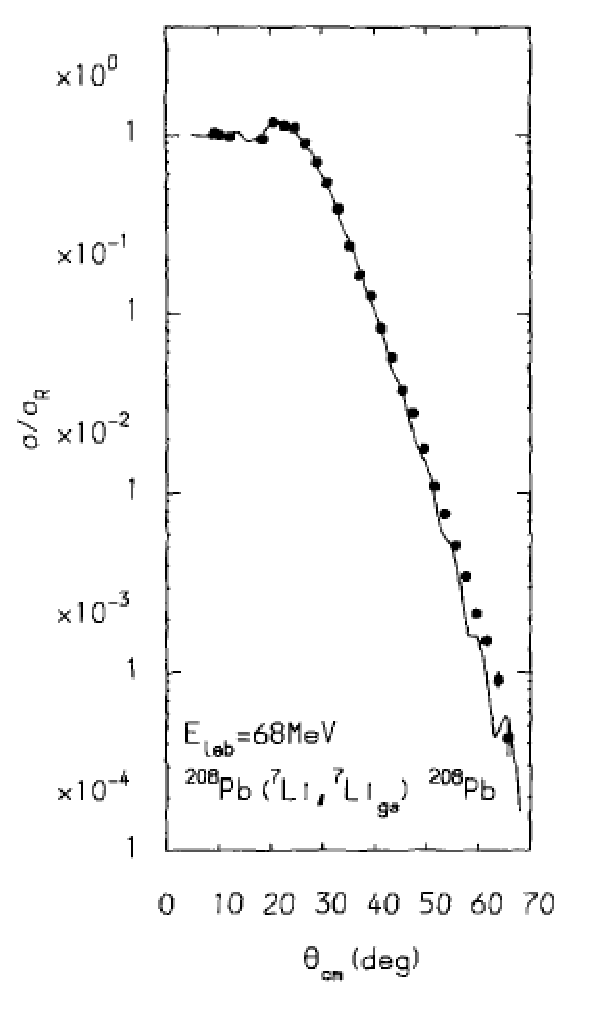
\includegraphics[height=5.5cm]{\images/li7pb_e70_el.eps} 

\includegraphics[height=5.5cm]{\images/li7pb_e70_inel.eps} 
\end{center}
\end{columns}
\end{frame}









%\subsection{The importance of the coupling to breakup channels}


% --------------------------------------------------------------------------------------
\slide{Application of the CC method to weakly-bound systems}


{\bf Example:}  {\blue Three-body calculation (p+n+\nuc{58}{Ni}) with Watanabe potential:}
$$
V_{dt}(\vecR)=\int d \vecr  \phi^*_\mathrm{gs}(\vecr) \left\{ V_{pt}(\br_{pt})  + V_{nt}(\br_{nt}) \right\}
 \phi_\mathrm{gs}(\vecr)
$$

\begin{columns}
\column{0.5\textwidth}
\begin{figure}{\par \resizebox*{0.8\textwidth}{!}
{\includegraphics{\images/dni_e80_1chan.eps}} \par}
\end{figure}
\column{0.4\textwidth}
\begin{center}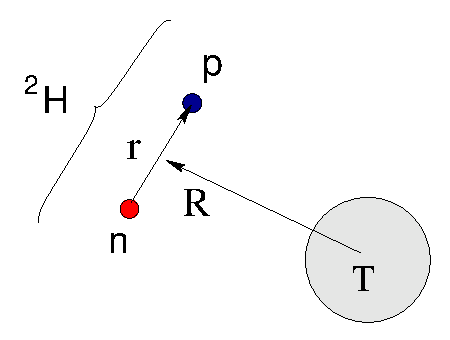
\includegraphics[height=2.5cm]{\images/dpb_coor.eps}\end{center}
\end{columns}


\ding{43}{\em \blue \small Three-body calculations omitting breakup channels fail to describe 
the experimental data.}
\end{frame}



% -------------------------------------------------------------------------------------------------
\slide{Bound versus scattering states}

\begin{columns}
\column{0.5\textwidth}
 \begin{figure}{\par \resizebox*{0.9\textwidth}{!}
 {\includegraphics{\images/deut2}} \par}
 \end{figure}
\column{0.5\textwidth}
Continuum wavefunctions: 
\bigskip

\psframebox[fillcolor=lightgreen,linecolor=blue,framearc=0.1,fillstyle=solid,framesep=-5pt]{
\parbox{0.9\columnwidth}{
$$ 
\varphi_{k,\ell jm}(\br) = {u_{k, \ell j} (r) \over r} [Y_{\ell}(\hat{r}) \otimes \chi_s  ]_{jm} 
$$
$$ 
\varepsilon=\frac{\hbar^2 k^2}{2 \mu} 
$$
}%parbox
}%psframe
\end{columns}

\pause
\vspace{0.5cm}

{\brick Unbound states are not suitable for CC calculations:} \\
\begin{itemize}
\item They have a continuous (infinite) distribution in energy.
\item Non-normalizable: $\langle u_{k,\ell s j}(r) | u_{k',\ell s j}(r) \rangle \propto \delta(k-k')$ 
\end{itemize}

\bigskip
\centering{ {\blue SOLUTION} $\Rightarrow$ {\blue continuum discretization}}

\end{frame}
% ------------------------------------------------------------------------------------------------


% -------------------------------------------------------------------------------------------------
\slide{The role of the continuum in the scattering of weakly bound nuclei}

\begin{itemize}

\item Continuum discretization method proposed  by G.H.~Rawitscher {\verde [ PRC9, 2210 (1974)]} and Farrell, Vincent and 
Austern {\verde [Ann.Phys.(New York) 96, 333 (1976)]}.
 \begin{figure}{\par \resizebox*{0.9\textwidth}{!}
 {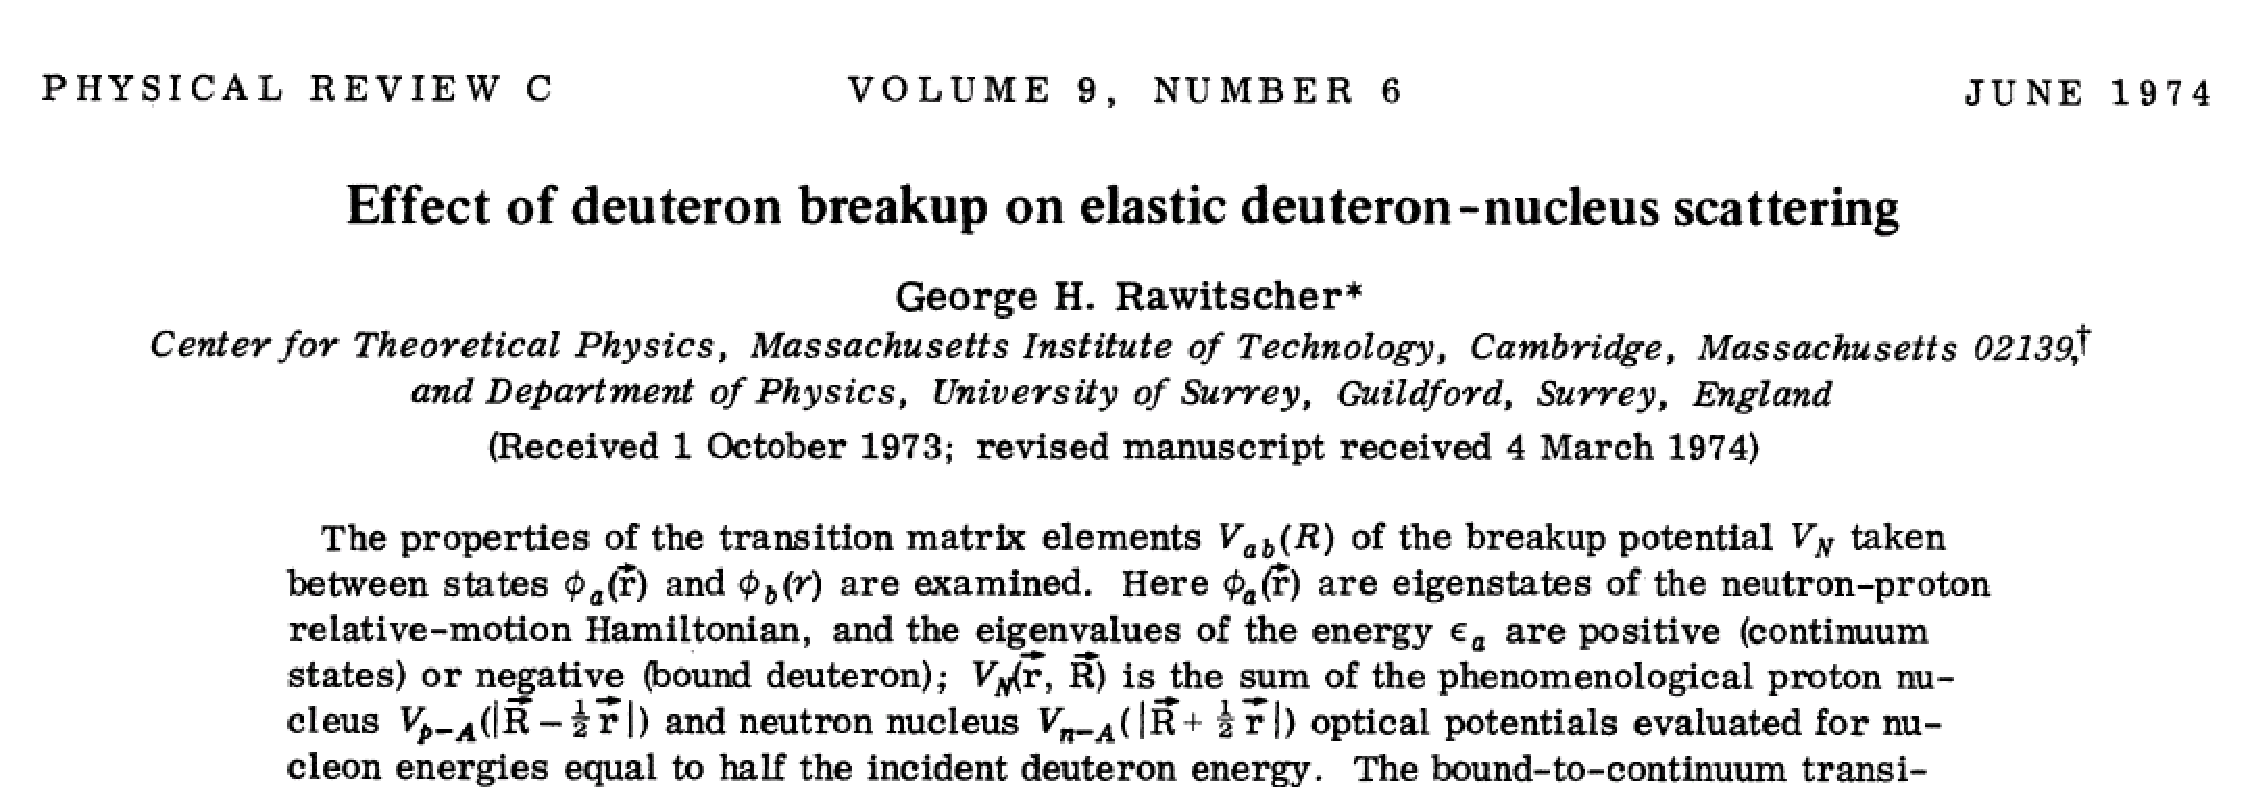
\includegraphics{\images/rawitscher.eps}} \par}
 \end{figure}


\item Full numerical implementation  by Kyushu group (Sakuragi, Yahiro, Kamimura, and co.): {\verde Prog.~Theor.~Phys.(Kyoto) 68, 322 (1982)}

\end{itemize} 
\end{frame}



% -------------------------------------------------------------------------------------------------
\slide{Continuum discretization for deuteron scattering}

\vspace{0.5cm}

%{\brick CDCC method} $\rightarrow$ continuum discretization: 

%{\blue Example:} discretization of the deuteron continuum in terms of energy bins.

%\begin{columns}
%\column{0.4\textwidth}
 \begin{figure}{\par \resizebox*{0.55\textwidth}{!}
 {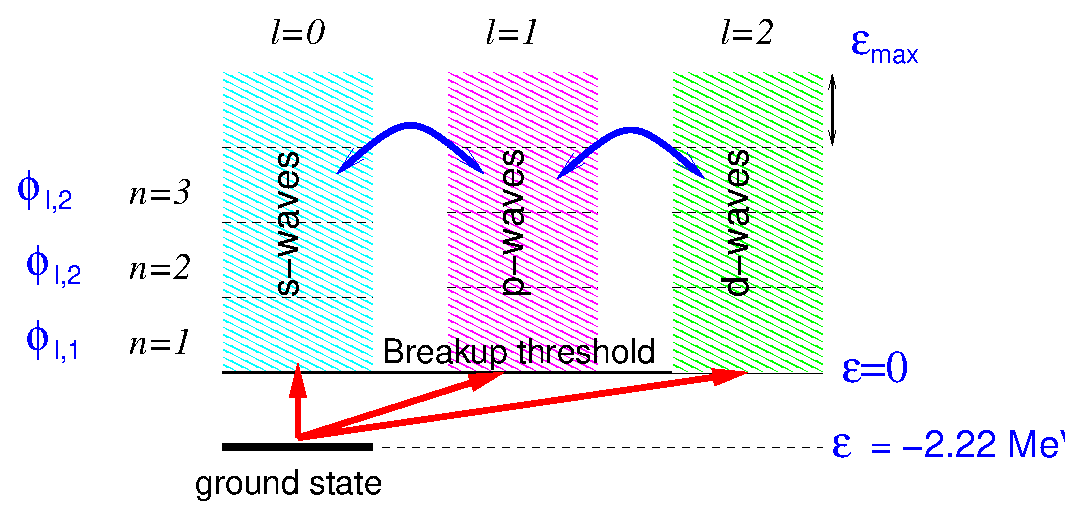
\includegraphics{\images/cdcc_deut.eps}} \par}
 \end{figure}
%\column{0.6\textwidth}
 \begin{itemize}
 \small
 \item[\ding{233}] Select a number of angular momenta ({\blue $\ell=0,\ldots,\ell_\mathrm{max}$}).
 \item[\ding{233}] For each $\ell$, set a maximum excitation energy {\blue $\varepsilon_\mathrm{max}$}.
 \item[\ding{233}] Divide the interval {\blue $\varepsilon=0-\varepsilon_\mathrm{max}$} in a set of sub-intervals ({\em \blue bins}).
  \item[\ding{233}] For each {\blue bin}, calculate a representative wavefunction. 
 \end{itemize}
%\end{columns}


\end{frame}
% --------------


% -------------------------------------------------------------------------------------------------
\slide{CDCC formalism: construction of the bin wavefunctions}

%\vspace{0.5cm}

{\blue Bin wavefunction:} $$\varphi^{[k_1,k_2]}_{\ell jm}(\br) =  {u^{[k_1,k_2]}_{\ell j}(r) \over r} [Y_{\ell}(\hat{r}) \otimes \chi_s  ]_{jm} 
\quad 
\quad 
[k_1,k_2] = \textrm{bin interval}
$$


\vspace{0.24cm}
\begin{columns}
\column{0.5\textwidth}
$$
\psframebox[linecolor=red,framearc=0.1]{
 u^{[k_1,k_2]}_{\ell sjm} (r) = \sqrt {\frac{2 }{\pi N}} ~~
            \int _ {k _ 1} ^ {k _ 2} w(k) u _{k,\ell sj} (r) dk
}%psfram
$$
\column{0.5\textwidth}
\begin{itemize}
\setlength{\itemsep}{0pt}
\item {\blue $k$}: linear momentum
\item {\blue $u _{k,\ell sj}(r)$}: scattering states (radial part)
\item {\blue $w(k)$}: weight function 
\end{itemize}
\end{columns}

\nccurve[linecolor=magenta,angleA=-90,angleB=155]{->}{F1}{T1}

\vspace{+0.2cm}

 \begin{figure}{\par \resizebox*{0.42\textwidth}{!}
 {\includegraphics{\images/wfbin.eps}} \par}
 \end{figure}

\end{frame}
% ------------------------------------------------------------------------------------------------



\begin{comment}

% --------------------------------------------------------------------------------------
\slide{Inclusion of the continuum in CC calculations: continuum discretization}

%\hspace{3.5cm}\rnode{A}{\psshadowbox[fillcolor=yellow,linecolor=black,framearc=0.2]{\blue Quantum Hamiltonian}}

\begin{center}\psshadowbox[fillcolor=yellow,linecolor=black,framearc=0.2]{\blue Quantum Hamiltonian}\end{center}


\vspace{1cm}
\begin{columns}
\column{0.5\linewidth}
%\hspace{0.5cm}\rnode[linecolor=red]{B1}
\begin{center}
{\psframebox{\parbox{3cm}{{\bf \verde Bound states}\\ - Discrete \\ - Finite \\ - Normalizable}}}
\end{center}
\column{0.5\linewidth}
\begin{center}
%\hspace{0.5cm}\rnode[linecolor=red]{B2}
{\psframebox{\parbox{4cm}{{\bf \verde Unbound states} \\ - Continuous \\ - Infinite \\ - Non-normalizable}}}
\end{center}
\end{columns}

%\ncline{->}{A}{B1}
%\ncline{->}{A}{B2}
%\nccurve[linecolor=red,angleA=-90,angleB=90]{->}{A}{B1}
%\nccurve[linecolor=red,angleA=-90,angleB=90]{->}{A}{B2}

\vspace{1cm}

{\bf \brick Continuum discretization:} represent the continuum by a finite set of square-integrable states

\begin{center}
\begin{tabular}{lcl}
%\small
{\bf \verde {\em True} continuum} & $\to$ & {\bf \verde Discretized continuum } \\
{Non normalizable}  &  $\to$ & {Normalizable} \\
{Continuous}         & $\to$ & {Discrete }
\end{tabular}
\end{center}
%}

\end{frame}
\end{comment}


\begin{comment}
% -------------------------------------------------------------------------------------------------
\slide{CDCC formalism}

\vspace{0.5cm}

%{\brick CDCC method} $\rightarrow$ continuum discretization: 
Coupled-Channels + Continuum discretization $\Rightarrow$ Continuum-Discretized Coupled-Channels (CDCC)!


{\brick Example:} discretization of the deuteron continuum in terms of energy bins.


 \begin{figure}{\par \resizebox*{0.65\textwidth}{!}
 {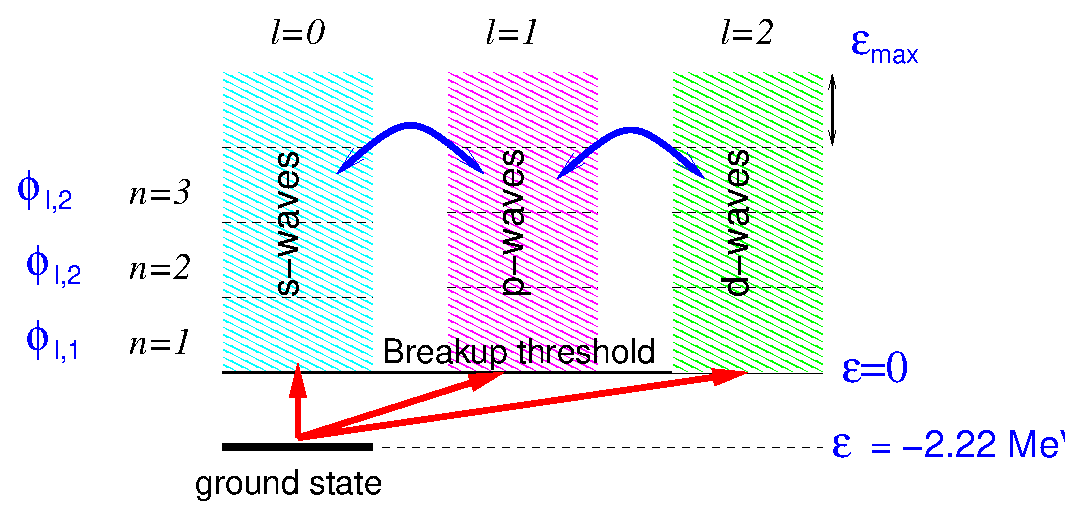
\includegraphics{\images/cdcc_deut}} \par}
 \end{figure}

\end{frame}
\end{comment}



\begin{comment}
% -------------------------------------------------------------------------------------------------
\slide{CDCC formalism: construction of the bin wavefunctions}

%\vspace{0.5cm}

{\brick Bin wavefunction:} 

\begin{center}
\psframebox[linecolor=red,framearc=0.1,framesep=0.0cm]{
\parbox{7.0cm}{
\begin{equation} 
\nonumber
{  u_{\ell sj,n} (r) = \sqrt {\frac{2 }{\pi N}} ~~
            \int _ {k _ 1} ^ {k _ 2} w(k) u _{\ell sj,k} (r) dk}
\end{equation}
}}%parbox
\end{center}

\begin{itemize}
\setlength{\itemsep}{0pt}
\item {\brick $k$}: linear momentum
\item {\brick $u _{\ell sj,k}$}: scattering states (radial part)
\item {\brick $w(k)$}: weight function 
\end{itemize}

\vspace{-0.2cm}

 \begin{figure}{\par \resizebox*{0.42\textwidth}{!}
 {\includegraphics{\images/wfbin.eps}} \par}
 \end{figure}

\end{frame}
% ------------------------------------------------------------------------------------------------
\end{comment}





% -------------------------------------------------------------------------------------------------
\slide{CDCC formalism for deuteron scattering}
% $\bullet$ Radial wavefunctions: 

%{\brick CDCC equations for radial wavefunctions:}

\begin{itemize}
\bc
\column{0.65\linewidth}
\gitem{Hamiltonian:}  $H = T_\bR   +  h_r(\br) + V_{pt}(\br_{pt}) + V_{nt}(\br_{nt})$ 

\gitem{Model wavefunction:}
 $$\Psi^{(+)}(\bR,\br)=\phi_{gs}(\br)\chi_{0}(\bR)+ \sum_{n>0}^{N} \phi_{n}(\br) \chi_{n}(\bR)$$

\column{0.35\linewidth}
\begin{figure}{\par \resizebox*{0.75\textwidth}{!}
 {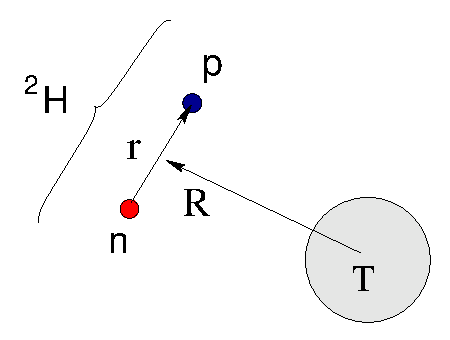
\includegraphics{\images/dpb_coor}} \par}
 \end{figure}
\ec

\gitem{Coupled equations:} $[H-E]\Psi(\bR,\br)=0$
$$
\psframebox[linecolor=red,framearc=0.1]{
\left[E-\varepsilon_{n}-T_R -V_{n,n}(\bR) \right] \chi_{n}(\bR)  = 
\sum_{n' \neq n} V_{n,n'}(\bR) \chi_{n'}(\bR) 
}%psframebox
$$

%-----------------
% Radial equations
% ----------------
% $$
% \psframebox[linecolor=red,framearc=0.1,framesep=2mm]{
%  \left [ 
% - \frac{\hbar^2 }{2 \mu} ~ \left ( \frac{d^2 }{ dR^2} - \frac{L(L+1)} {R^2} \right )
% + \epsilon_n - E \right ]
% f _ {\alpha J} (R)  + \sum _ {\alpha '} 
% i ^ {L ' - L} ~ V^J _{\alpha:\alpha'}(R)  f_{\alpha' J} (R) =0 
% }
% $$
% {\brick $\alpha$}= $\{L,\ell,s,j,n\}$ 


\gitem{Transition potentials:}
$$
%\psframebox[linecolor=red,framearc=0.2,framesep=2mm]{
V_{n;n^\prime}(\vecR) = 
\int d \vecr  \phi_n^{*}(\vecr)
	\left[ V_{pt} (\vecR +\frac{\vecr}{2}) + V_{nt} (\vecR-\frac{\vecr}{2})\right] 
 \phi_{n^\prime}(\vecr) 
%}
$$

\end{itemize}

\end{frame}
% -------------------------------------------------------------------------------------------------


% ------------------------------------------------------------------------------------------------
\slide{Application of the CDCC formalism: d+ $^{58}$Ni}

%\psframebox[fillcolor=green!15,linecolor=blue,framearc=0.1]{
\begin{center}\small Coupled-Channels + Continuum discretization \end{center}
%}%
\begin{center}$\Downarrow$ \end{center}
\begin{center}
\psframebox[fillcolor=green!15,linecolor=blue,framearc=0.1]{
\small Continuum-Discretized Coupled-Channels (CDCC) 
}%psframe
\end{center}

\begin{columns}
\column{0.5\textwidth}
\begin{figure}{\par \resizebox*{0.8\textwidth}{!}
    {\includegraphics{\images/dni_e80_kd.eps}} \par}
\end{figure}
\column{0.5\textwidth}
\begin{center}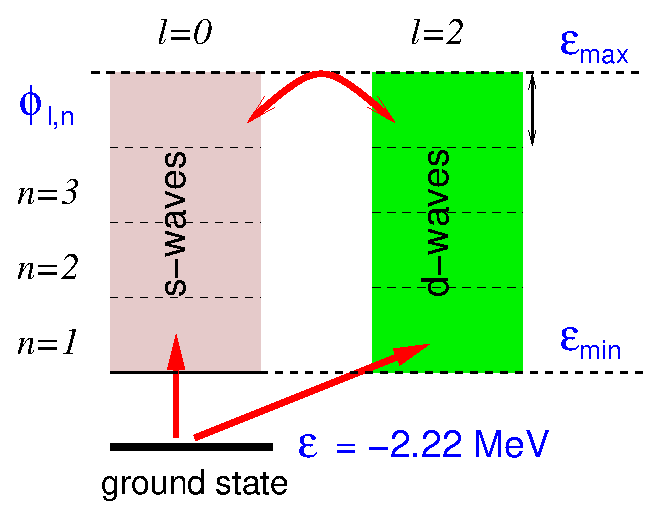
\includegraphics[width=0.75\textwidth]{\images/cdcc_deut_sd.eps} \end{center}

\end{columns}

% \ding{43} No continuum $\Rightarrow$ retain only the Watanabe potential: 
% $$
% V_{00}(\vecR)=\int d \vecr  \phi_\mathrm{gs}(\vecr) \left( V_{pt}  + V_{nt}\right)
%  \phi_\mathrm{gs}(\vecr)
% $$

\bigskip

\ding{43}{\it \small Coupling to breakup channels has a important effect on the reaction dynamics}

\end{frame}





% --------------------------------------------------------------------------------------
\slide{Application of the CDCC method: \nuc{6}{Li} and \nuc{6}{He} scattering}

\begin{itemize}
\item[\ding{43}]{\verde The CDCC has been also applied to nuclei with a cluster structure:}
\item \nuc{6}{Li}=$\alpha$ + d ~~~~ ($S_{\alpha,d}$=1.47~MeV)
\item \nuc{11}{Be}=\nuc{10}{Be} + n ($S_n$=0.504~MeV)
\end{itemize}

\medskip
\bc
\column{0.5\linewidth}
\begin{figure}{\par \resizebox*{0.85\textwidth}{!}
{\includegraphics{\images/li6ca_el_cdcc.eps}} \par}
\end{figure}
\column{0.5\linewidth}
\begin{figure}{\par \resizebox*{0.85\textwidth}{!}
{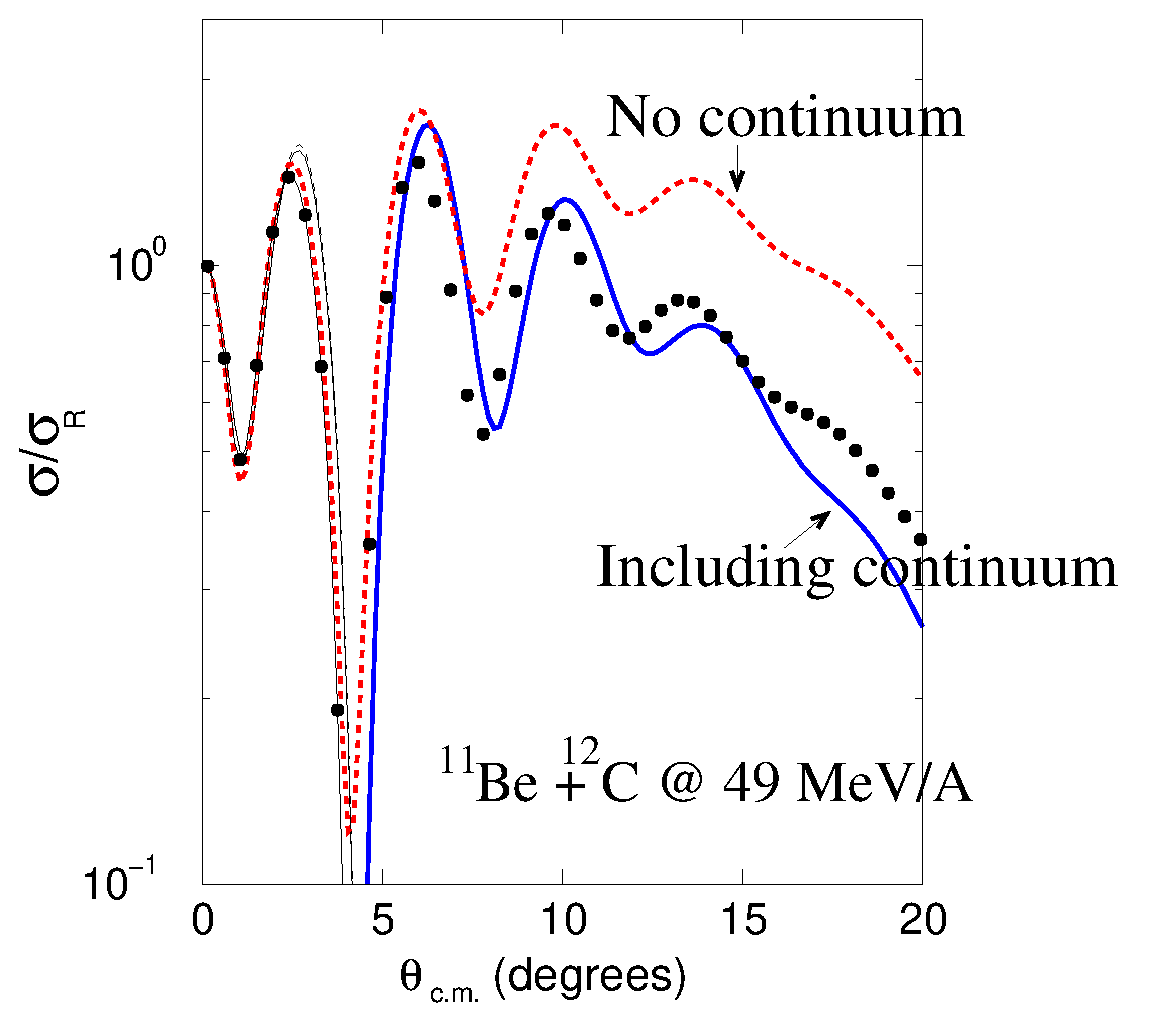
\includegraphics{\images/BeC.eps}} \par}
\end{figure}
\ec

%\pause
%\ding{43} {\verde \em \small In Fraunhofer scattering the presence of the continuum produces a reduction of the elastic  cross section} 

\end{frame}



\begin{comment}
% ---------------------------------------------------------------------------------------------------
\begin{wideslide}[toc=,bm=] {Extension to 3-body projectiles}
%\onslide*{2}{
\begin{itemize}
\item[\ding{43}]{\verde The CDCC has been recently extended to 3-body projectiles:}
\item {\bf Eg:} \nuc{6}{He}=$\alpha$ + n + n  \quad (M.Rodr\'{\i}guez-Gallardo et al,PRC 77, 064609 (2008))
\end{itemize}


\begin{figure}{\par \resizebox*{0.4\textwidth}{!}
  {\includegraphics{\images/he6pb_e27_el.eps}} \par}
  \end{figure}
%}%onslide
\pause 
\ding{43} {\verde \em \small In Fresnel scattering the coupling to the continuum supresses the interference peaks} 
\end{frame}
% --------------------------------------------------------------------------------------------------
\end{comment}






\begin{comment}
% ---------------------------------------------------------------------------------------------------
\slide{The importance of transfer/breakup channels}

\begin{itemize}
\item For ``normal'' nuclei, the elastic channel is dominant. 
\item For weakly-bound nuclei, transfer/breakup channels become very important.
\end{itemize} 

{\bf Example:} $\alpha$ particles arising in \nuc{6}{He}+\nuc{208}{Pb}

\begin{figure}{\par \resizebox*{0.40\textwidth}{!}
{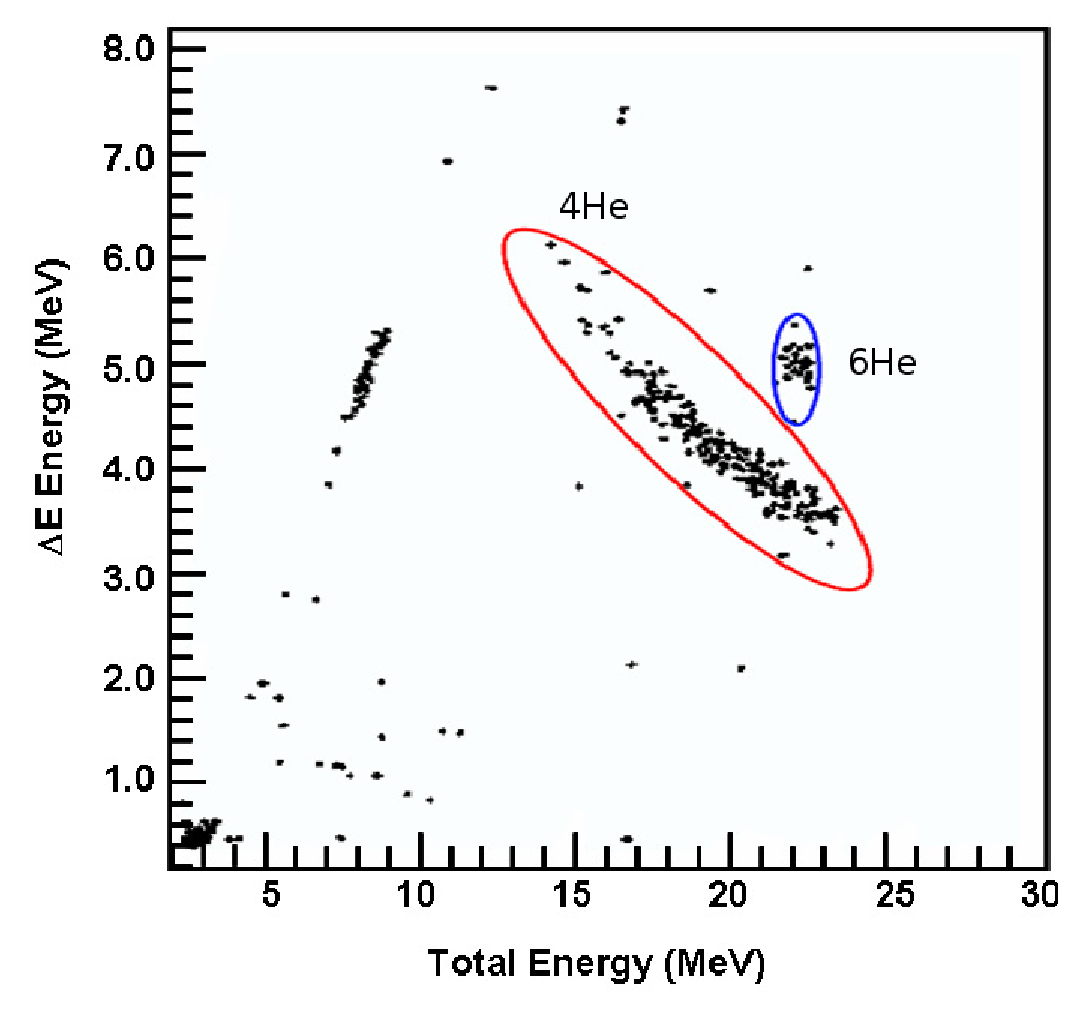
\includegraphics{\images/bidim-22MeV-new2.eps}} \par}
\end{figure}

\end{frame}
\end{comment}






%%%%%%%%%%%%%%%%%%%%%%%%%%%%%%%%%%%%%%%%%%%%%%%%%%%%%%%%%%%%%%%%%%%%%%%%%%%%%%%%%%%%%%%%%%%%%%%%%%%%%%%%%





%-----------------------------------------------------------------------------------------------------
\subsection{Recent extensions of the CDCC method}
%-----------------------------------------------------------------------------------------------------
%\slide{}
%\begin{center}
%\psframebox[fillcolor=green!10,linecolor=blue,framearc=0.1,fillstyle=solid,framesep=5pt]{
%Recent extensions of the CDCC method
%}%psframe
%\end{center} 
%\end{frame}

% ---------------------------------------------------------------------------------------------------
\slide{Extension to 3-body projectiles}

\begin{figure}{\par \resizebox*{0.4\textwidth}{!}
  {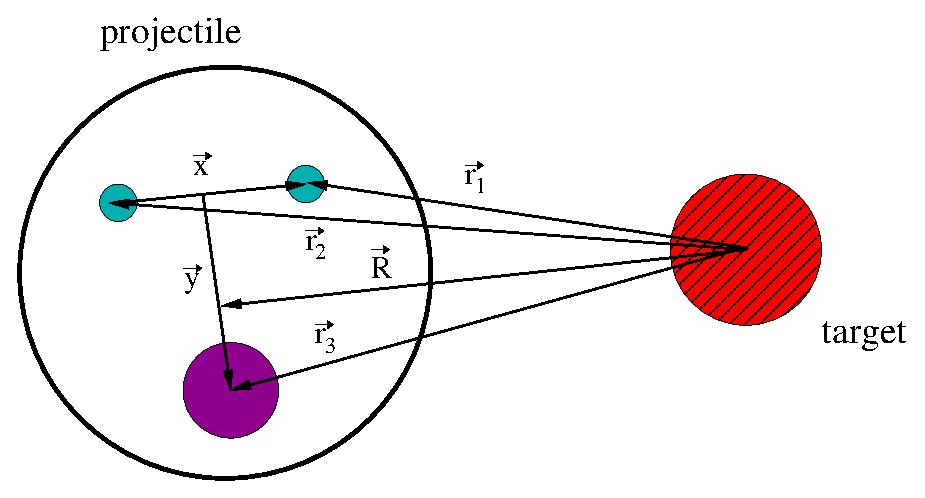
\includegraphics{\images/4c.eps}} \par}
\end{figure}


To extend the  CDCC formalism, one needs to evaluate the new coupling potentials:
$$
\psframebox[linecolor=red,framearc=0.2,framesep=1mm]{
V_{n;n^\prime}(\vecR) = 
\int d \vecr  \, \phi_n^{*}(\bx,\by)
	\left\{ V_{nt} (\br_{1}) + V_{nt} (\br_{2})  + V_{\alpha t} (\br_{3}) \right\}
 \phi_{n^\prime}(\bx,\by) 
}
$$
\ding{43} $\phi_n(\bx,\by)$ three-body WFs for bound and continuum states: hyperspherical coordinates, Faddeev, etc (difficult to calculate!)


\end{frame}





% ------------------------------------------------------------------------------------------------
\slide{Four-body CDCC calculations for $^6$He scattering}

\begin{center}\includegraphics[height=4.5cm]{\images/he6pb_e22_4bcdcc.eps} \end{center}

N.b.: 1-channel potential considers only g.s. $\rightarrow$ g.s. coupling potential:
$$
\psframebox[fillcolor=green!10,linecolor=blue,framearc=0.1,framesep=5pt]{
V_{00}(\vecR) = 
\int d \vecr  \, \phi_\mathrm{g.s.}^{*}(\bx,\by)
	\left\{ V_{nt} (\br_{1}) + V_{nt} (\br_{2})  + V_{ct} (\br_{3}) \right\}
 \phi_\mathrm{g.s.}(\bx,\by) 
}%psframe
$$


\scriptsize
Data (LLN): \scita{S\'anchez-Ben\'{\i}tez et al, NPA 803, 30 (2008) L. Acosta et al, PRC 84, 044604 (2011)} \\
Calculations:  \scita{Rodr\'iguez-Gallardo et al, PRC 80, 051601 (2009)}

\end{frame}








% ------------------------------------------------------------------------------------------------
\slide{Polarization potential from CDCC calculations}

\small
\begin{columns}
\column{0.5\textwidth}

\begin{center}\includegraphics[height=6.0cm]{\images/he6pb_pol_coul.eps} \end{center}

\column{0.5\textwidth}

\begin{center}\includegraphics[height=6.0cm]{\images/he6pb_pol_nuc.eps} \end{center}

% \cita{M~Cubero et al, PRL109, 262701 (2012)} \\
% \cita{J.~Fern\'andez-Garc\'{\i}a et al, PRL110,142701(2013)}

\end{columns}

\bi
\small
\item Polarization potentials are {\blue long-ranged}. 
\item Both {\blue nuclear} and {\blue Coulomb} couplings are important. 
%({\blue long-range absorption})
\ei

\end{frame}








% ----------------------------------------------------------------------------------
\subsection{Non-elastic breakup}
%-----------------------------------------------------------------------------------------
\slide{}
\begin{center}
\psframebox[fillcolor=green!10,linecolor=blue,framearc=0.1,fillstyle=solid,framesep=5pt]{
The problem of inclusive breakup 
}%psframe
\end{center} 
\end{frame}




% ------------------------------------------------------------------------------------------------
\slide{$\alpha$ production in $^{6}$He scattering}

$$
\psframebox[fillcolor=yellow,linecolor=red,framearc=0.1]{
{\rm ^{6}{He} + ^{208}{Pb} \rightarrow  \alpha + X}
}
$$

\small
\begin{columns}
\column{0.5\textwidth}

\begin{center}\includegraphics[height=4.5cm]{\images/he6pb_e22_4bcdcc.eps} \end{center}

\column{0.5\textwidth}
\begin{center}\includegraphics[height=4.5cm]{\images/he6pb_e22_pbu.eps} \end{center}
\end{columns}

\bigskip

\ding{43}{\blue CDCC reproduces elastic scattering, but not {\blue inclusive} $\alpha$'s. }



%\psframebox[fillcolor=blue!10,fillstyle=solid,framearc=0.2,framesep=2pt]{
%\parbox{0.95\columnwidth}{%
%\small
%CDCC reproduces elastic scattering, but not {\blue inclusive} $\alpha$'s. 
%}}

\end{frame}



%-------------------------------------------------
\slide{\small Evaluation of the inclusive breakup}
 \begin{center}
%\includegraphics[width=0.8\columnwidth]{\images/dA_chans.eps}\end{center}
\begin{columns}
\column{0.6\textwidth}
 \begin{center}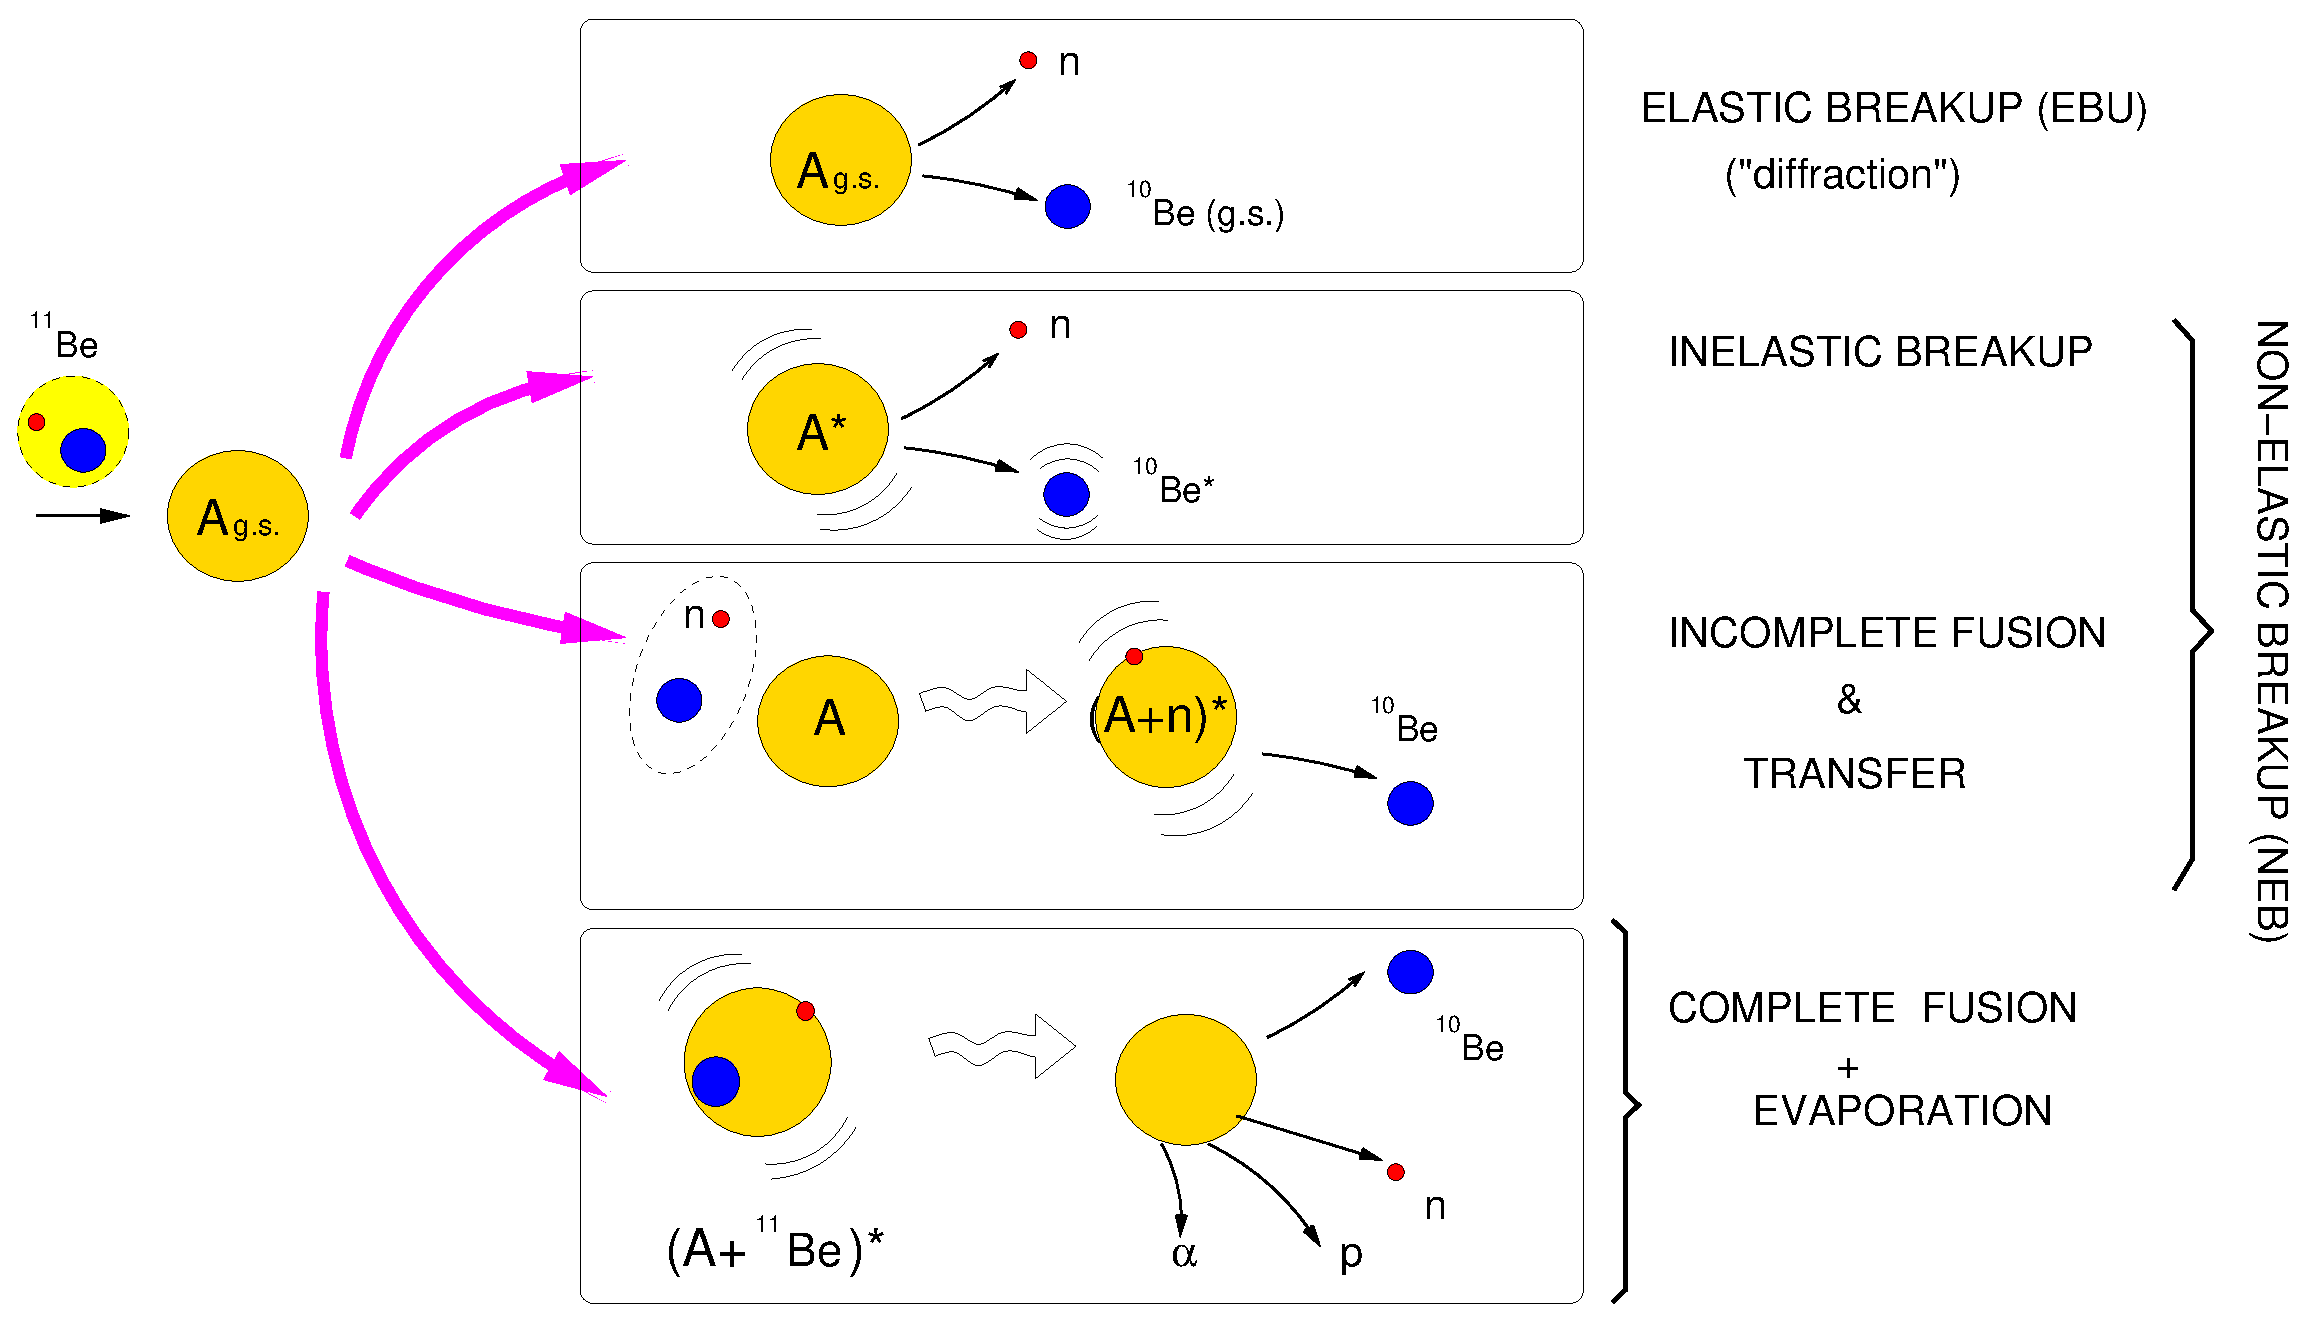
\includegraphics[height=4.5cm]{\images/be11_chans.eps}\end{center}
\column{0.4\textwidth}
\only<2->{
\begin{center} \includegraphics[height=4.5cm]{\images/be11_methods.eps} \end{center}
}%only
\end{columns}
\end{center}
\vspace{0.3cm}

\begin{itemize}
\small
\item [\ding{233}]{\small  For a reaction of the form  $a(=b+x)  + A \rightarrow b + \textrm{anything}$ }
$$
%\psframebox[linecolor=red,framearc=0.25,framesep=0.1cm]{
\psframebox[linecolor=red,fillcolor=orange!10,fillstyle=solid,framearc=0.2]{
\sigma_b =  \sigma_{EBU} + \sigma_{NEB} + \sigma_{CN} 
}
$$  
\item[\ding{233}] {\small CDCC provides only the EBU part ($\sigma_{NEB}$ \& $\sigma_{CN}$ out of CDCC modelspace}
\end{itemize}
\end{frame}




%------------------------------------------------------------------------
\slide{Evidence of NEB contributions in inclusive ($^6$Li,$\alpha$X) }

\begin{columns}
\column{0.5\textwidth} %------------------------------------------------------------------------
\psframebox[fillcolor=LightBlue!50,fillstyle=solid,framearc=0.2]{
 \parbox{5cm}{
 \begin{center}{\brick \scriptsize  $^{6}$Li+$^{209}$Bi @ 32 MeV} \\
 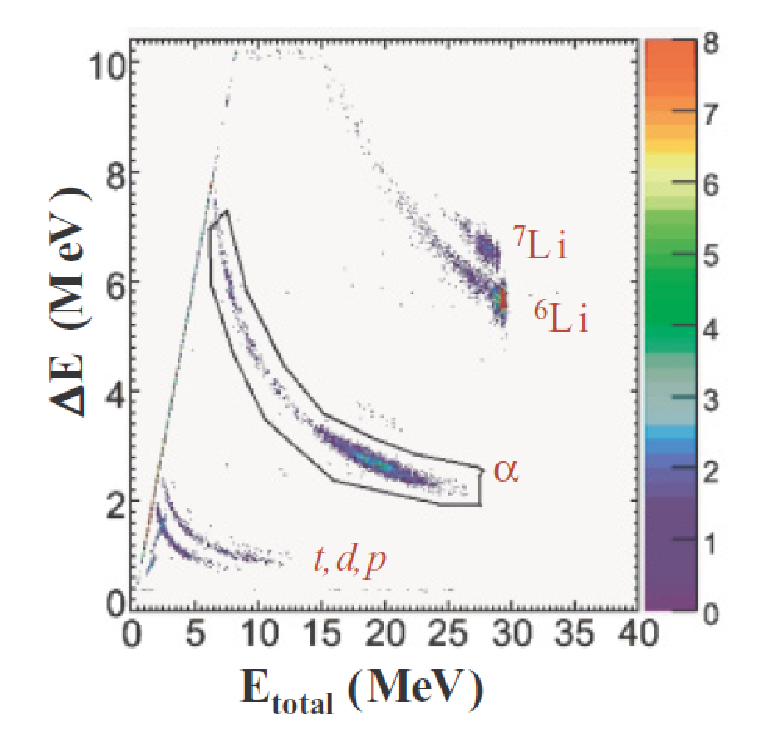
\includegraphics[width=4.5cm]{\images/li6bi_bidim.eps} \\
 \scriptsize
 Santra {\it et al}, PRC85,014612(2008) \end{center}
  }%parbox
 }%psframe
\column{0.5\textwidth} %------------------------------------------------------------------------
If elastic breakup were the dominant mechanism, we would expect $N_\alpha \approx N_{d}$ but,
experimentally, one finds  $N_\alpha \gg N_{d}$
\end{columns}


\end{frame}


%------------------------------------------------------------------------
\slide{Evidence of NEB contributions in inclusive $^{209}$Bi($^6$Li,$\alpha$)X }

\begin{columns}[t]
\column{0.5\textwidth}
\only<1>{
\begin{center}{\brick Elastic scattering} \end{center}
\begin{center}\includegraphics[height=6.0cm]{\images/li6bi_el.eps} \end{center}
%(\scriptsize 3b-CDCC requires reduced d+$^{209}$Bi absorption $\rightarrow$ Ogata's talk)
}%only
\column{0.5\textwidth}
\only<1>{
\begin{center}{\brick Inclusive $\alpha$'s } \end{center}
\begin{center}\includegraphics[height=6.0cm]{\images/li6bi_dsdw_ebu.eps} \end{center}
}%only
\end{columns}
\end{frame}




%-------------------------------------------------------------------------------------------------
\slide{Explicit evaluation of inclusive breakup in Ichimura-Austern-Vincent model}

\bi 
\bitem{Inclusive breakup:} 
$$
\psframebox[linecolor=red,fillstyle=solid,framearc=0.2]{
 a(=b+x) + A \rightarrow b + (x+A)^* 
}%
$$

\psframebox[fillcolor=red!10,framearc=0.2,framesep=4pt]{
\parbox{0.85\columnwidth}{%
{\it  Inclusion of all relevant $x+A$ channels is not feasible in general $\Rightarrow$ use closed-form models}
}%parbox
}%psframe


\bitem{Inclusive differential cross section: $\sigma^\mathrm{BU}_{b} = \sigma^\mathrm{EBU}_b +  \sigma^\mathrm{NEB}_b$}:
\bi
\item $\sigma^\mathrm{EBU}_b$ is breakup leaving $A$ in g.s. (e.g.\ CDCC)
\item  $\sigma^\mathrm{NEB}_b$ corresponds to non-elastic x+A processes and can be calculated as the absorption in the $x+A_{gs}$ channel:
$$
\psframebox[linecolor=red,fillcolor=orange!10,fillstyle=solid,framearc=0.2]{
\frac{d\sigma^\mathrm{NEB}}{d \Omega_b d E_b} = - \frac{2}{\hbar v_a} \rho_b(E_b) \langle \varphi^{(0)}_x | W_{xA} | \varphi^{(0)}_x \rangle
}%psframe
\quad
\textrm{(optical theorem)}
$$

where $\varphi^{(0)}_x$ describes $x-A$ scattering following $a \rightarrow b+x$ dissociation: 
$$
\psframebox[linecolor=red,fillcolor=orange!10,fillstyle=solid,framearc=0.2]{
 [K_x + U_{xA} -E_x] \varphi^{(0)}_{x}(\br_x) = ( \chi_b^{(-)} | V_{bx} | \chi_{aA} \phi_{a}  \rangle
}
$$
\ei

\ei
\end{frame}





%-------------------------------------------------------------------------------------------------
\slide{Application to $^{209}$Bi ($^{6}$Li+,$\alpha$ + X) }
\begin{columns}%[t]
\column{0.5\textwidth}
\begin{center}{\brick Elastic scattering} \end{center}
\begin{center}\includegraphics[height=6.5cm]{\images/li6bi_el.eps} \end{center}

\column{0.5\textwidth}
\begin{center}{\brick Inclusive $\alpha$'s } \end{center}
\begin{center}\includegraphics[height=6.5cm]{\images/li6bi_dsdw_rem.eps} \end{center}
\end{columns}
\end{frame}



%-------------------------------------------------------------------------------------------------
\begin{frame}[t]
\frametitle{\small $^{6}$Li+$^{209}$Bi: incident energy dependence of cross sections}
%Decomposition of the reaction cross section:
\only<1>{ \begin{center}\includegraphics[height=5.0cm]{\images/li6bi_sigedep_1.eps} \end{center} }
\only<2>{ \begin{center}\includegraphics[height=5.0cm]{\images/li6bi_sigedep_2.eps} \end{center} }
\only<3>{ \begin{center}\includegraphics[height=5.0cm]{\images/li6bi_sigedep_3.eps} \end{center} }
\only<4>{ \begin{center}\includegraphics[height=5.0cm]{\images/li6bi_sigedep_4.eps} \end{center} }
\only<5>{ \begin{center}\includegraphics[height=5.0cm]{\images/li6bi_sigedep_5.eps} \end{center} }
\only<6>{ \begin{center}\includegraphics[height=5.0cm]{\images/li6bi_sigedep.eps} \end{center} }

\only<6>{
%Our preliminary calculations indicate that:
$$
\psframebox[linecolor=red,framearc=0.25,framesep=0.1cm]{
\sigma_{reac} \approx \sigma_{\alpha+d} (EBU)+ \sigma_{\alpha}(NBU) + \sigma_{d} (NBU)  + \sigma(CF)
}%psframe
$$
%\ding{43} {\it \verde Suggests small transfer cross sections (for this reaction!)}
}%only

\end{frame}






%--------------------------------------------------------
\slide{Application to the $^{7}$Be case }
%--------------------------------------------------------

Data: Mazzocco {\it et al}:  \ding{43} $\sigma_\alpha \approx 5 \sigma_\mathrm{3He}$

\begin{center}\includegraphics[height=4.5cm]{\images/7Be58Ni.eps} \end{center}

\end{frame}







% ------------------------------------------------------------------
\subsection{Exploring the continuum with breakup reactions}
% ------------------------------------------------------------------
\slide{}
\begin{center}
\psframebox[fillcolor=green!10,linecolor=blue,framearc=0.1,fillstyle=solid,framesep=5pt]{
Exploring the continuum with breakup reactions
}%psframe
\end{center} 
\end{frame}



%----------------------------
\slide{Exclusive breakup measurements of halo nuclei}

{\bf Example:} $^{11}$Be+$^{208}$Pb $\rightarrow$ $^{10}$Be+ n+ $^{208}$Pb measured at RIKEN (69 MeV/u).

\cita{Fukuda et al, PRC70, 054606 (2004))}

\bigskip
\begin{center}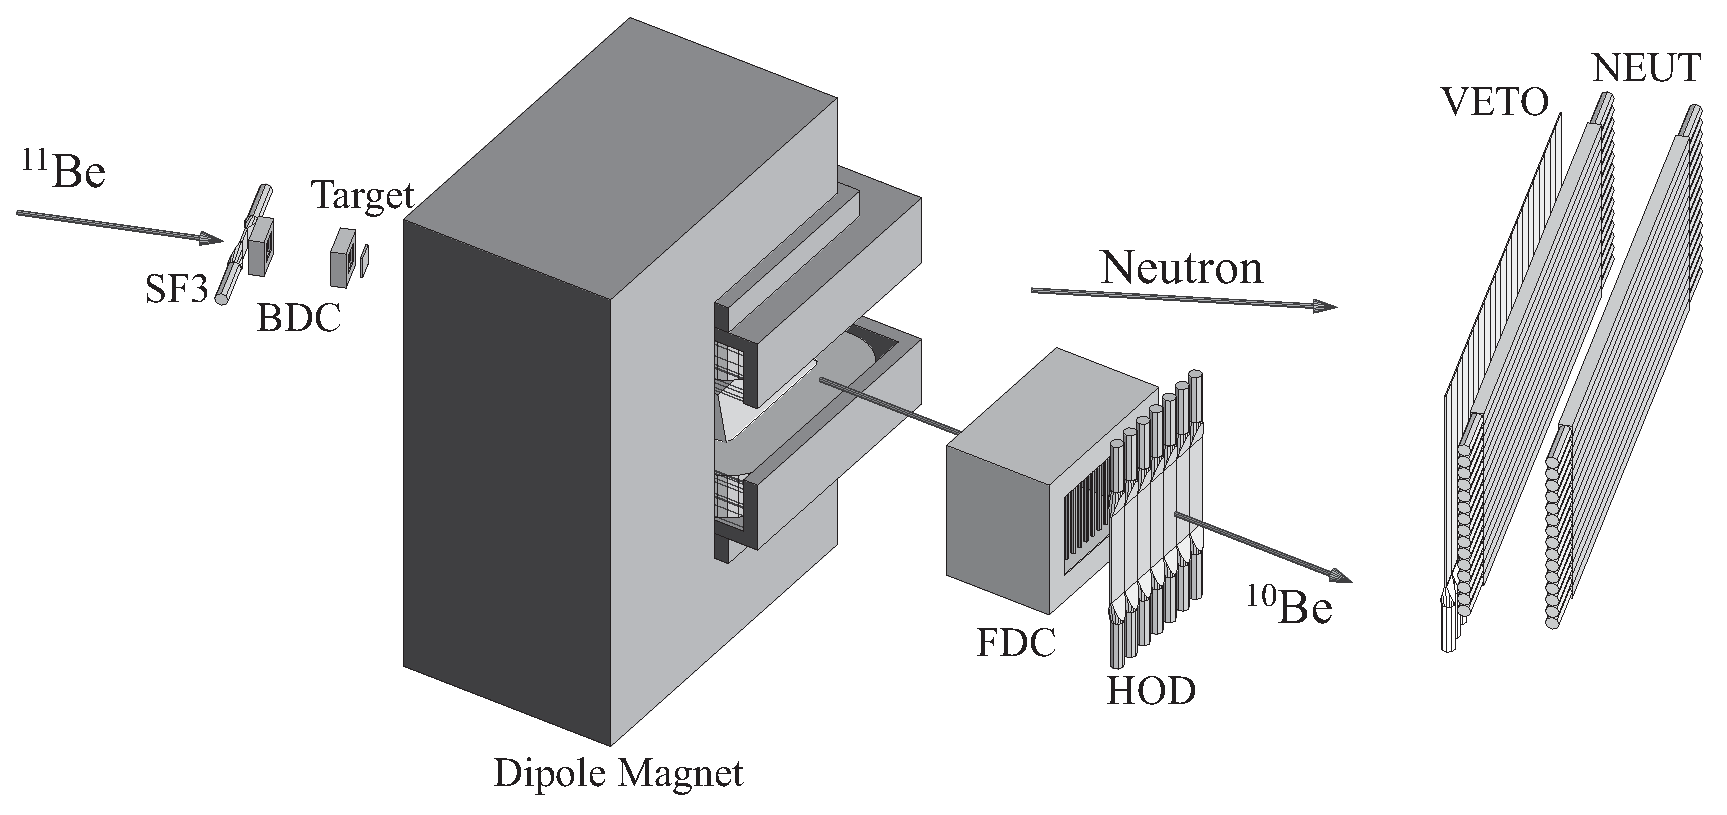
\includegraphics[height=3.0cm]{\images/fukuda_fig1.eps} \end{center}
\begin{itemize}
\item[\ding{43}] $^{11}$Be excitation energy can be reconstructed from core-neutron coincidences ({\em invariant mass method})
\end{itemize}

\end{frame}


% JAT SLIDE
%\slide{Strong response to electric fields}
%\begin{center}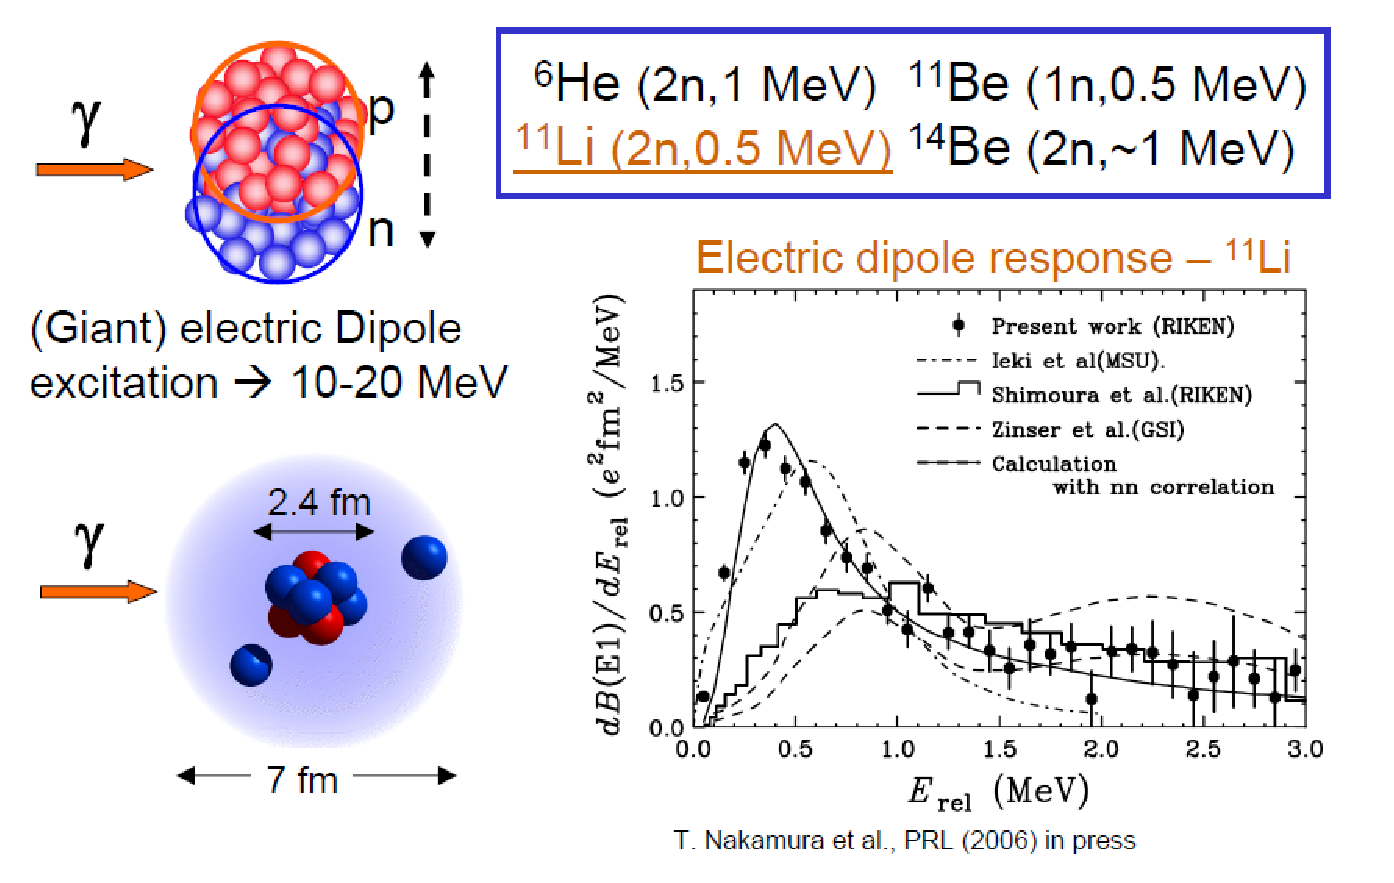
\includegraphics[height=0.85\textheight]{\images/e1_response.eps}\end{center}
%\end{frame}


%-------------------------------------------------
\slide{Dominance of $E1$ coupling }

\bi
\small
\item $^{11}$Be+$^{208}$Pb $\rightarrow$ $^{10}$Be+ n+ $^{208}$Pb measured at RIKEN (69 MeV/u).
\item CDCC calculations include nuclear and Coulomb couplings to all orders. 
\ei

\begin{center}\includegraphics[height=0.55\textheight]{\images/be11pb_dsdw_erel5.eps}\end{center}

\bi
\small
\item[\ding{43}] For $\theta_\mathrm{c.m.} \ll$, the breakup is dominated by g.s. to continuum E1 transitions ($1/2^+ \rightarrow 1/2^-,3/2^-$).  
\item[\ding{43}] For pure E1 transitions, we can resort to the simpler semiclassical theory of Coulomb excitation.  
\ei

\end{frame}


%--------------------------------------------------
\slide{Semiclassical 1st order E$\lambda$ excitation (Alder \& Winther)}

\begin{itemize}
\item For E$\lambda$ excitation to bound states ($0 \rightarrow n$)
$$
\psframebox[fillcolor=green!10,linecolor=blue,framearc=0.1]{
\left( {d \sigma \over d \Omega}\right)_{0\rightarrow n}= \left({ Z_t  e^2 \over   \hbar v}\right)^2
{B(E \lambda, 0 \to n) \over  e^2 a_0^{2 \lambda-2}} f_\lambda(\theta,\xi)
}%psframe
\quad
%\xi_{0 \rightarrow n} = \frac{(E_n-E_0)}{\hbar} \tau_{col} \approx \frac{(E_n-E_0)}{\hbar} \frac{a_0}{v} 
\xi_{0 \rightarrow n} =  \frac{(E_n-E_0)}{\hbar} \frac{a_0}{v} 
$$


\item Halo nuclei are weakly bound $\Rightarrow$ excitation occurs to unbound (continuum) states:
$$
\psframebox[fillcolor=green!10,linecolor=blue,framearc=0.1]{
 \frac{d \sigma(E\lambda)}{d \Omega d E} = \left({ Z_t  e^2 \over   \hbar v}\right)^2
{1 \over  e^2 a_0^{2 \lambda-2}}
\frac{dB(E \lambda)}{dE} 
{df_\lambda(\theta,\xi) \over d\Omega}
}%psframe
$$
%\item[\ding{43}] ${df_\lambda(\theta,\xi) / d\Omega}$ is a well-defined analytic function. 

\item[\ding{43}] ${dB(E \lambda)}/{dE}$ can be extracted from small-angle Coulomb dissociation data.  
$$
\psframebox[fillcolor=green!10,linecolor=blue,framearc=0.1,fillstyle=solid]{
\frac{d\sigma}{dE} (\theta < \theta_\mathrm{max}) = 
\int_{0}^{\theta_\mathrm{max}}  \frac{d \sigma(E\lambda)}{d \Omega d E} d\Omega
\propto \frac{dB(E \lambda)}{dE}  
% \int_{0}^{\theta_\mathrm{max}} {df_\lambda(\theta,\xi) \over d\Omega}
}%
$$

\end{itemize}
\end{frame}





%------------------------------------ 11Be+208Pb ----------------------
\slide{Extracting $B(E1)$ of $^{11}$Be from  $^{11}$Be+$^{208}$Pb Coulomb dissociation}

%Eg: $^{11}$Be+$^{208}$Pb at RIKEN \cita{Fukuda et al, PRC70, 054606 (2004))}

\bc
\column{.5\textwidth}
\begin{center}  \includegraphics[height=3.25cm]{\images/be11pb_dsdw_epm.eps} \end{center}

\column{.5\textwidth}
\small
$$
\psframebox[fillcolor=green!10,linecolor=blue,framearc=0.1]{
 \frac{d \sigma(E\lambda)}{d \Omega d E} = \left({ Z_t  e^2 \over   \hbar v}\right)^2
{1 \over  e^2 a_0^{2 \lambda-2}}
\frac{dB(E \lambda)}{dE} 
{df_\lambda(\theta,\xi) \over d\Omega}
}%psframe
$$

($dB(E1)/dE$ from a two-body model, $^{10}$Be+n) 
\ec

\pause

\bc
\column{.42\textwidth}
%\begin{center}  \includegraphics[height=3.5cm]{\images/be11pb_dsde_sp.eps} \end{center}
\begin{center}  \includegraphics[height=3.5cm]{\images/be11pb_dsde_epm.eps} \end{center}

\column{.12\textwidth}

$$\frac{dB(E \lambda)}{dE}  \propto  \frac{d\sigma}{dE} $$  


\includegraphics[width=0.8\columnwidth]{\images/arrow-green.eps}

\column{.42\textwidth}
\begin{center}  \includegraphics[height=3.5cm]{\images/be11_dbde.eps} \end{center}
\ec

See \scita{Fukuda et al, PRC70, 054606 (2004))}
\end{frame}

%-------------------- 19C+208Pb ------------------------
%\slide{$^{11}$Be+$^{208}$Pb at RIKEN}
%\begin{center}  \includegraphics[width=0.85\textwidth]{\images/c19pb_dsde.eps} \end{center}
%\cita{Nakamura et al, Phys. Rev. Lett. 83 1112 (1999)}
%\end{frame}

\slide{The importance of multistep couplings}

$^{11}$Be+$^{197}$Au $\rightarrow$ $^{10}$Be + n +$^{197}$Au

\begin{center}
\includegraphics[height=6.5cm]{\images/be11au_bu3.eps}
\end{center}

\end{frame}




% ----------------------------------------------------------------------------------
%\subsection{Accessing continuum structures: resonant breakup}


%\slide{}
%\begin{center}
%\psframebox[fillcolor=green!10,linecolor=blue,framearc=0.1,fillstyle=solid,framesep=5pt]{
%Exploring continuum structures
%}%psframe
%\end{center} 
%\end{frame}

%\subsection{Structures in the continuum}
% ---------------------------------------------------------------------------------------------------
\slide{Exploring structures in the continuum}

%\vspace{1cm}

The continuum spectrum is not ``homogeneous''; it contains in general energy regions with 
special structures, such as {resonances} and {virtual} states

%\begin{itemize}
%\item Resonances
%\item Virtual states
%\end{itemize}

\begin{center}\includegraphics[angle=0,width=0.3\textwidth]{\images/be11_spectrum_crop.eps} \end{center}

\pause 
\ding{43} {\em \verde These structures may (or may not!) show up in reaction observables}

\end{frame}


%---------------------------------------------------------------------------------------------------
\slide{What is a resonance?}

\begin{itemize}

\item It is a {\blue pole} of the S-matrix in the complex energy plane. 

\item It is a structure on the continuum which may, or may not, produce a {\blue maximum in the cross section}, depending on the reaction mechanism and the phase space available.


\item The resonance occurs in the range of energies for which the {\blue phase shift
is close to $\pi/2$}.

\item In this range of energies, the continuum wavefunctions have a 
 {\blue large probability of being in the radial range of the potential}.

\item The continuum wavefunctions are {\blue not square normalizable}. However, a
normalized ``bin'' of wavefunctions can be constructed to represent the 
resonance.

\end{itemize}

\end{frame}



%------------------------------------------------------------------------------------
\slide{Distinctive features of a resonance}

In the energy  range of the resonance, the continuum wavefunctions have a 
 large probability of being within the range of the potential.

\bigskip
\bc
\column{0.5\linewidth}
\center{ \includegraphics[width=4.8cm]{\images/am5.eps}}
(Courtesy of C.~Dasso) 
\column{0.5\linewidth}
\center{ \includegraphics[width=5.2cm]{\images/be11_reswf.eps}}
\ec
\end{frame}



%------------------------------------------------------------------------------------
\slide{Distinctive features of a resonance}
The decay of the resonance is also behind the $\alpha$-decay phenomenon: 

\bigskip
\bc
\column{0.5\linewidth}
\center{ \includegraphics[width=6cm]{\images/alpha-tunneling.eps}}
\column{0.5\linewidth}
\center{ \includegraphics[width=5.0cm]{\images/alpha-decay.eps}}
\ec

\end{frame}





\begin{comment}
% --------------------------------------------------------------------------------------------------
\slide{What is a resonance?}

\begin{itemize}
\setlength{\itemsep}{14pt}

\gitem{Definition 1:} (Experimentalist)  It is a  maximum in the cross section as a function of the energy 

\gitem{Definition 2.1:} (Theoretician)  It is a pole on the  S-matrix

\gitem{Definition 2.2:} (Another theoretician)  It's a solution of the Schr\"rodinger equation with a growing 
 exponential asymptotic behaviour.
 
\gitem{Definition 3:}  It is a structure on the continuum (which may show up in some reaction observables)
\end{itemize}
\end{frame}


% --------------------------------------------------------------------------------------------------
\begin{wideslide}[toc=,bm=]{What is a resonance?}



\textcolor{blue}{Definition 1: (Experimentalist) 
It is a  maximum in the cross section as a function of the energy}

\bigskip

{\bf Eg:} \nuc{9}{Li} + d $\to$ \nuc{10}{Li} + p

\center{\includegraphics[width=6cm]{\images/bu_vsE_data.eps}}

{\verde \em Is this bump a resonance?}
\end{frame}


%------------------------------------------------------------------------------------
\begin{wideslide}[toc=,bm=]{}

%\small

{\bf...but}

\begin{itemize}

\item Not all the maxima in the cross section can be associated to resonances.
Coupling to a non-resonant continuum produces a maximum at some energy, which
is related to the size of the system, and the properties of the interaction.

\item For weakly bound systems, resonances can be very broad (1 MeV), and occur
at relatively low excitation energies. It is not clear, a priori, whether a
bump in the cross section is a signature of a genuine resonance, or not.

\end{itemize}

\end{frame}


%-------------------------------------------------------------------------------
\begin{wideslide}[toc=,bm=]{What is a resonance?}


 \textcolor{blue}{Definition 2: (Theoretician)  It is a pole on the 
S-matrix (eg. of the n+\nuc{9}{Li} system)}

 \bigskip

{\bf ...but}

\begin{itemize}

\item The fact that there is a pole in the S-matrix in the complex E plane 
does not allow, by itself, to calculate the cross section to the resonance.

\item The wave function corresponding to a pole in the complex E-plane 
is not square-normalizable.

\item Finding poles in a complex energy-plane for multi-channel 
or three-body systems is difficult. 

\end{itemize}

\end{frame}


%---------------------------------------------------------------------------------------------------
\begin{wideslide}[toc=,bm=]{What is a resonance?}

\textcolor{blue}{Definition 3: It is a structure on the continuum}

which may, or may not, produce a maximum in the cross section, depending on the reaction mechanism and the phase space available.

\begin{itemize}

\item The resonance occurs in the range of energies for which the phase shift
is close to $\pi/2$.

\item In this range of energies, the continuum wavefunctions have a 
 large probability of being in the radial range of the potential.

\item The continuum wavefunctions are not square normalizable. However, a
normalized ``bin'' of wavefunctions can be constructed to represent the 
resonance.

\end{itemize}

%\center{ \includegraphics[width=7cm]{\images/bu_vsE_vs100vp67.eps}}


\end{frame}






\begin{comment}
%------------------------------------------------------------------
\begin{wideslide}{What is a resonance?}
 \textcolor{blue}{Definition 4: It is a square-normalizable state,
which is not stationary}

but it does maintain its caracter during a time longer than the collision time.

\begin{itemize}

\item The time evolution of the resonance leads to a reduction within the 
range of the potential, given by $\exp(-\Gamma t/\hbar)$, plus an outgoing
component.

\item The non-stationary nature of the state can be neglected during the 
collision if $\Gamma \ll \hbar/T_c $. 

\item The square normalizable state can be expanded in terms of ``true'' 
continuum states, to obtain the cross section distribution.


\end{itemize}

\end{frame}






%-------------------------------------------------------------------
\end{comment}


%---------------------------------------------------------------------------------------------
\slide{Resonances and phase-shifts}

\only<1>{
\begin{figure}{\par \resizebox*{0.7\textwidth}{!}
{\includegraphics{\images/smat.eps}} \par}
%{\includegraphics{\images/smatrix}} \par}
\end{figure}

}%

\only<2>{
\begin{figure}{\par \resizebox*{0.8\textwidth}{!}
{\includegraphics{\images/delta_res}} \par}
\end{figure}
({\scriptsize \it borrowed from J.~Tostevin})
}

\end{frame}
% ----------------------------------------------------------------------------------


% ----------------------------------------------------------------------------------
\slide{Populating resonances by ``inelastic scattering'': \nuc{11}{Be}+\nuc{12}{C}}


\nuc{11}{Be}+\nuc{12}{C} $\rightarrow$ (\nuc{10}{Be}+n) + \nuc{12}{C}  \quad {\verde Fukuda et al, Phys. Rev. C70 (2004) 054606)}

\bc
\column{0.5\textwidth}
\begin{center}
\includegraphics[width=0.7\textwidth]{\images/be11c12_erel_crop.eps} \\
\includegraphics[angle=-90,width=0.7\textwidth]{\images/be11_spectrum_crop.eps} 
\end{center}

\column{0.5\textwidth}
\begin{center} DWBA calculations \end{center}
\begin{center}\includegraphics[width=0.9\columnwidth]{\images/fukuda_fig5.eps} \end{center}
\ec

\end{frame}







%---------------------------------------------------------------------------------------------
%\begin{wideslide}[toc=, bm=]{Spectroscopy to unbound states: \nuc{9}{Li}(d,p)\nuc{10}{Li} case}
\slide{Virtual states}
\begin{itemize}
\item Neutrons in $s$-wave cannot produce resonat states (no barrier)
\item Still, they can exhibit distinctive structures, characterized by a rapid increase of the phase-shift near zero energy ({\brick virtual states}). This behaviour is commonly characterized in terms of the {\brick scattering length}:
$$
\psframebox[fillcolor=yellow,linecolor=red,framearc=0.1]{
 {\blue  a_s= -\lim_{k \to 0} \tan \frac{\delta (k)}{k} }
}%psframe
$$

\end{itemize}

\begin{columns}
\column{0.4\linewidth}
\begin{figure}{\par \resizebox*{1.1\textwidth}{!}
{\includegraphics{\images/li9nn_psh_s12.eps}} \par}
\end{figure}
\column{0.4\linewidth}
\begin{figure}{\par \resizebox*{0.85\textwidth}{!}
{\includegraphics{\images/slength.eps}} \par}
\end{figure}
\end{columns}
\end{frame}



\begin{comment}
%------------------------------------------------------------------------------------
\slide{Virtual states (continued)}
 Virtual states are non-normalizable solutions of the Schrodinger equation for a imaginary momentum $-i |k|$ and negative energy: $E_s = \hbar^2 (-i |k|)^2/2\mu= - \hbar^2 |k|^2/2\mu$. 

\begin{columns}
\column{0.5\textwidth}
\begin{figure}{\par \resizebox*{0.85\textwidth}{!}
{\includegraphics{\images/virtual-g1b}} \par}
\end{figure}
\column{0.5\textwidth}
\begin{figure}{\par \resizebox*{0.9\textwidth}{!}
{\includegraphics{\images/li9n_swell}} \par}
\end{figure}
\end{columns}%twocolumn

\end{frame}
\end{comment}

%--------------------------------------------------------------------------------
\slide{Resonances and virtual states in the complex energy/momentum plane}

{\small Virtual states are non-normalizable solutions of the Schrodinger equation for a imaginary momentum $-i |k|$ and negative energy: $E_s = \hbar^2 (-i |k|)^2/2\mu= - \hbar^2 |k|^2/2\mu$. }

\begin{figure}{\par \resizebox*{0.65\textwidth}{!}
{\includegraphics{\images/complex_poles.eps}} \par}
\end{figure}

({\scriptsize \it figure borrowed from Thompson \& Nunes' book})

\end{frame}


%----------------------------------------------------------------------------------
\slide{Bound vs virtual (anti-bound) states in the N-N system}

\begin{figure}{\par \resizebox*{0.7\textwidth}{!}
{\includegraphics{\images/3s1_1s0.eps}} \par}
\end{figure}

\begin{itemize} 
\item $p-n$: $\delta(E) \xrightarrow{E\rightarrow0 } \pi$ $\Rightarrow$ one-bound state (deuteron)
\item $p-p$, $n-n$:  no bound states, but they do have an anti-bound (virtual) state. 
\item $p-p$: $\delta$ becomes negative for large $E$ $\Rightarrow$ evidence of repulsive core!
\end{itemize}
\end{frame}



\begin{comment}
%--------------------------------------------------------------------------------
\slide{Appearance of a virtual state in \nuc{10}{Li}=\nuc{9}{Li}+n:}
\bigskip

\begin{columns}
\column{0.5\textwidth}
\begin{figure}{\par \resizebox*{1.0\textwidth}{!}
{\includegraphics{\images/virtual-g1b}} \par}
\end{figure}
\column{0.5\textwidth}
\begin{figure}{\par \resizebox*{0.9\textwidth}{!}
{\includegraphics{\images/li9n_swell}} \par}
\end{figure}
\end{columns}%twocolumn

\end{frame}




%---------------------------------------------------------------------------------------------
\slide{Virtual state in $^{10}$Li}

% \begin{center}
% {\blue \psframebox[fillcolor=yellow]{$V_s$ (virtual state)}}
% \end{center}

%{\blue \psframebox{Virtual state}}

\begin{columns}
\column{0.4\linewidth}
\begin{figure}{\par \resizebox*{1.1\textwidth}{!}
{\includegraphics{\images/li9nn_psh_s12.eps}} \par}
\end{figure}

\psframebox[fillcolor=yellow,linecolor=red,framearc=0.1]{
\parbox{4.5cm}{
Scattering length: \\
 {\blue  $$a_s= -\lim_{k \to 0} \tan \frac{\delta (k)}{k} $$}
}%parbox
}%frame

\column{0.4\linewidth}
\begin{figure}{\par \resizebox*{0.85\textwidth}{!}
{\includegraphics{\images/slength.eps}} \par}
\end{figure}
\end{columns}
\end{frame}
\end{comment}








\subsection{Inclusion of core excitation}
%---------------------------------------------------------------------------------------------
\slide{Inclusion of core excitation}
\begin{center}
\psframebox[fillcolor=green!10,linecolor=blue,framearc=0.1,fillstyle=solid,framesep=5pt]{
Beyond the strict few-body model: inclusion of {\it core} excitations
}%psframe
\end{center} 
\end{frame}


%-------------------------------------------------------------------------------------
\slide{\small Beyond the strict few-body picture: the effect of core excitation}
\vspace{1cm}
\begin{center}
\mishadowbox{To what extent can one ignore the dynamics of the core?}

\vspace{1cm}

\includegraphics[height=2.5cm]{\images/be11t_mic.eps} 

\bigskip

%(work done with R. Crespo and R. C. Johnson)
\end{center}
\end{frame}
% ---------------------------------------------------------------------------------------


%----------------------------------------------------------------------------------------
\slide{Core excitation in structure: $^{11}$Be case}

\bi 
\setlength{\itemsep}{14pt}
\item {\brick Strict single-particle model:}
\begin{minipage}[c]{.6\textwidth}
\small
$$
| ^{11}{\rm Be} (1/2^+) \rangle =  \mid \shalfzero \rangle
$$
\end{minipage}
\begin{minipage}[c]{.29\textwidth}
\begin{center}\includegraphics[width=0.72\columnwidth]{\images/be11_capas_inert.eps}  \end{center}
\end{minipage}

\pause 

\item {\brick Core-excitation model:}
\small
$$
| ^{11}{\rm Be} (1/2^+) \rangle =  {\blue a} \mid \shalfzero \rangle+ \nonumber 
           {\blue b} \mid \dhalftwo \rangle + \ldots
$$
\begin{center}
\includegraphics[width=0.75\columnwidth]{\images/be11_capas_corex2.eps}  
\end{center}

%\item[]  
{\blue $a$}, {\blue $b$}  = spectroscopic amplitudes  
\ei

\end{frame}



%-------------------------------------------------------------------------------------
\slide{Core excitation in reactions: {\it frozen-halo} picture}

\begin{minipage}[c]{.6\textwidth}
$$ 
\psframebox[linecolor=red,fillcolor=orange!10,fillstyle=solid,framearc=0.2]{
\Psi_{JM}(\vec{r},{\magenta \xi}) =   
\left[  { \varphi^J_{\ell,j}(\vec{r})}  \otimes \Phi_{I}({\magenta \xi}) \right]_{JM} 
}%psframe
$$
\bi
\item[\ding{233}] ${ \varphi^J_{\ell,j}(\vec{r})}$= valence particle wavefunction
\item[\ding{233}] $\Phi_{I}({\magenta \xi})$= core wavefunction ({\it frozen})
\ei
\end{minipage}
\begin{minipage}[c]{.29\textwidth}
\begin{center}\includegraphics[width=0.9\columnwidth]{\images/be11_cvdef.eps}  \end{center}
\end{minipage}

\vspace{0.5cm}

\begin{minipage}[t]{.55\textwidth}
\only<1>{\begin{center}\includegraphics[width=0.65\columnwidth]{\images/be11_spect_sp.eps} \end{center}}
\only<2>{\begin{center}\includegraphics[width=0.75\columnwidth]{\images/be11_spect_sptrans.eps} \end{center}}
\end{minipage}
\begin{minipage}[t]{.44\textwidth}
\begin{center}\includegraphics[width=0.8\columnwidth]{\images/be11pb_valence.eps} \end{center}
\end{minipage}

\end{frame}


%-------------------------------------------------------------------------------------
\slide{Core excitation mechanism in breakup}

\begin{minipage}[c]{.6\textwidth}
$$
\psframebox[linecolor=red,fillcolor=orange!10,fillstyle=solid,framearc=0.2]{
\Psi_{JM}(\vec{r},{\magenta \xi}) =  \sum_{\ell,j,I} 
\left[  { \varphi^J_{\ell,j,I}(\vec{r})}  \otimes \Phi_{I}({\magenta \xi}) \right]_{JM} 
}%psframe
$$
%\bi
%\item[\ding{233}] ${ \varphi^J_{\ell,j}(\vec{r})}$= valence particle wavefunction
%\item[\ding{233}] $\Phi_{I}({\magenta \xi})$= core wavefunction
%\ei
\end{minipage}
\begin{minipage}[c]{.29\textwidth}
\begin{center}\includegraphics[width=0.85\columnwidth]{\images/be11_cvdef.eps}  \end{center}
\end{minipage}

%\pause 
\vspace{0.5cm}

\begin{minipage}[t]{.6\textwidth}
\only<1>{\begin{center}\includegraphics[width=0.9\columnwidth]{\images/be11_spect_cmix.eps} \end{center}}
\only<2>{\begin{center}\includegraphics[width=0.9\columnwidth]{\images/be11_spect_cmix_trans.eps} \end{center}}
\end{minipage}
\begin{minipage}[t]{.39\textwidth}
\begin{center}\includegraphics[width=0.8\columnwidth]{\images/be11pb_corex.eps} \end{center}
\end{minipage}
\only<2>{\ding{43} \em \small Core excitation/deexcitation during the reaction contributes to the inelastic \& breakup probabilities} 
%\only<2>{\ding{43} \em \small Dynamic core excitation favors population of states with same parity as ground state} 
\end{frame}




%----------------------------------------------------------------------
\slide{CDCC with core excitations (XCDCC)}
\begin{itemize}
\item {\blue Standard CDCC.} $\Rightarrow$  uses coupling potentials:
$$
\psframebox[linecolor=red,framearc=0.1,framesep=0.2cm]{
V_{\alpha;\alpha^\prime}(\vecR) = 
\langle \Psi^{\alpha'}_{J' M'}(\vec{r}) |
 V_{vt}(r_{vt}) + V_{ct}( r_{ct})| 
 \Psi^{\alpha}_{J M}(\vec{r})  \rangle
}%psframe
$$

\item {\blue  Extended CDCC} $\Rightarrow$ uses generalized coupling potentials
$$
\psframebox[linecolor=red,framearc=0.1,framesep=0.2cm]{
V_{\alpha;\alpha^\prime}(\vecR) = 
\langle \Psi^{\alpha'}_{J' M'}(\vec{r},{\magenta {\magenta \xi}}) |
 V_{vt}(r_{vt}) + V_{ct}( r_{ct},{\magenta {\magenta \xi}})| 
 \Psi^{\alpha}_{J M}(\vec{r},{\magenta {\magenta \xi}})  \rangle
}%psframe
$$
%\cita{Summers {\em et al}, PRC74 (2006) 014606, PRC76 (2007) 014611}
\cita{Summers {\em et al}, PRC74 (2006) 014606} (bin discretization) \\
\cita{R.~de Diego {\em et al}, PRC89, 064609 (2014)} (PS discretization) 

\end{itemize}

\end{frame}





%----------------------------
\begin{frame}[t]
\frametitle{\small Evidence of reaction-induced core excitations in p($^{11}$Be,p') at 64 MeV/u (MSU)}

Data: \scita{Shrivastava et al, PLB596 (2004) 54} (MSU)
\begin{columns}[c]

%\column{0.3\textwidth}
%\only<1,2>{
%\begin{center}\includegraphics[height=3.5cm]{\images/be11_spectrum3.eps} \end{center}
%}


\column{0.5\textwidth}
\only<1>{
\begin{center}\includegraphics[height=5.0cm]{\images/shriv_spec_regions_test.eps}  \\

 \end{center}
}%onslide

\column{0.5\textwidth}
\scriptsize


\only<1>{
%\begin{center}\includegraphics[height=5.0cm]{\images/be11p_dsdw_def.eps} \end{center} % DWBA
\begin{center}\includegraphics[height=5.0cm]{\images/be11p_dsdw_xcdcc.eps} \\
\scita{R.de Diego et al, PRC85, 054613 (2014)} \end{center}
}%only
\end{columns}%twocol

\vspace{0.25cm}

%\only<1>{
%\scriptsize
%\bi
%\item $E_{rel}$=0--2.5 MeV contains $5/2^+$ resonance (expected {\blue single-particle} mechanism)
%\item $E_{rel}$=2.5--5 MeV contains $3/2^+$ resonance (expected {\blue core excitation} mechanism)
%\ei
%}%only

%\vspace{0.25cm}

\only<1>{
\psframebox[fillcolor=blue!10,fillstyle=solid,framearc=0.2,framesep=4pt]{
\parbox{0.9\columnwidth}{%
\small
\ding{233} {\scriptsize Dynamic core excitations gives additional (and significant!) contributions to breakup}
}%parbox
}%psframe


}%only
\end{frame}



%----------------------------
\begin{frame}[t]
\frametitle{\small Dominance of {\it dynamical} core excitations in p($^{19}$C,$^{18}$C+n)p resonant breakup}

%Data: \scita{Satou et al, PLB660 (2008) 320} (RIKEN)
\begin{columns}[c]

\column{0.5\textwidth}
\only<1,2>{
\begin{center}\includegraphics[height=5.0cm]{\images/satou_fig1_mod.eps} \\
\scita{Satou et al, PLB660 (2008) 320} (RIKEN) \end{center}
}%onslide


\column{0.5\textwidth}
\scriptsize


\only<1>{
\begin{center}\includegraphics[height=4.0cm]{\images/c19spectrum.eps}  \end{center}
}%only


\only<2>{
%\begin{center}\includegraphics[height=5.0cm]{\images/be11p_dsdw_def.eps} \end{center} % DWBA
\begin{center}\includegraphics[height=4.0cm]{\images/c19pdsdw_conv_6.eps} \\
\scita{J.A.~Lay et al, PRC 94, 021602 (2016)} \end{center}
}%only
\end{columns}%twocol

\vspace{0.25cm}


\vspace{0.25cm}

\only<2>{
\psframebox[fillcolor=blue!10,fillstyle=solid,framearc=0.2,framesep=4pt]{
\parbox{0.9\columnwidth}{%
\small
\ding{233} {\scriptsize The core-excitation mechanism gives the dominant contribution to the cross section}
}%parbox
}%psframe

}%only
\end{frame}



% ----------------------------------------------------------------------------------
\slide{Application to $^{11}{\rm Be}+^{12}{\rm C}$: valence/core interplay}

\begin{columns}[t]
\column{0.4\textwidth}
%\twocolumn[lcolwidth=0.4\linewidth,rcolwidth=0.6\linewidth,colsep=0cm,frsep=0pt]{
\begin{center}\includegraphics[width=0.95\linewidth]{\images/be11c_dsdw_be12b_ren.eps} \end{center}

\column{0.6\textwidth}

{\small

\begin{itemize}
\item Interference effects between {\blue valence} \& {\red core} mechanisms are essential to explain the shape.
\item This sensitivity  can provide constraints on weights of different configurations. 
\end{itemize}

}%small  

\end{columns}%twocolumn
\end{frame}





\subsection{Comparison with the Faddeev formalism}
%-----------------------------------------------------------------------------------------------------
\slide{}
\begin{center}
\psframebox[fillcolor=green!10,linecolor=blue,framearc=0.1,fillstyle=solid,framesep=5pt]{
Comparison with the Faddeev formalism
}%psframe
\end{center} 
\end{frame}



\begin{comment}
% ------------------------------------------------------------------------------------------------
\slide{CDCC versus Faddeev}

\begin{itemize}
\item The {\em exact} solution of a three-body scattering problem is formally given by the 
      Faddeev equations.

 \begin{center}\includegraphics[height=1.75cm]{\images/be11p_3jacobi.eps} \end{center}

\item The CDCC method can be derived as an approximated solution of the Faddeev equations 
      in a trucated model space ({\verde Austern,Yahiro,Kawai, PRL63 (1989) 2649})

\item For light systems, Faddeev equations can be now solved, so a comparison with CDCC 
      is possible. 
\end{itemize}
\end{frame}
\end{comment}

% ------------------------------------------------------------------------------------------------
\slide{Some words by Ludwig Faddeev on his own work}

\begin{center} %\hspace{6cm}
\includegraphics[height=2.5cm]{\images/Faddeev_n.eps}
\end{center}

{\it ``(...)The treatment of the {\blue quantum scattering theory for the system of three particles}, based on the integral equations, now bearing my name, brought me my first success. The work was highly appreciated by the specialists in {\blue nuclear physics}. The attention of mathematicians came later and now the theory of many body quantum scattering is an active subject of modern mathematical physics. However, personally I estimate higher my solution of the overdetermined many dimensional inverse problem for the Schroedinger operator with local potential(...)'' }

\bigskip

\hspace{3cm}\cita{L.~Faddeev, Autobiography written for the ``Shaw Prize''}

\end{frame}



% ------------------------------------------------------------------------------------------------
\slide{CDCC versus Faddeev}

{\verde Austern,Yahiro,Kawai, PRL63, 2649 (1989)}:
\begin{itemize}
\item The CDCC method can be derived as an approximation of the Faddeev equations
      in a {\blue truncated model space} for a {\blue selected Jacobi set}.

\begin{center} $$\Psi^\mathrm{Fad} = \Psi_1 + \Psi_2 + \Psi_3 \approx \Psi_1 $$\end{center}

\begin{center}\includegraphics[height=2.5cm]{\images/be11p_3jacobi_circle.eps} \end{center}
%}

\item The CDCC solution should converge to Faddeev, when the model space is increased (never tested in practice!).
\end{itemize}
%\item For light systems, Faddeev equations can be now solved, so a comparison with CDCC  is possible. 

\end{frame}




\slide{Testing CDCC for elastic scattering: d+\nuc{58}{Ni} at 80 MeV}
%\begin{center}\includegraphics[height=5cm]{\\images/dni_e80_kd.eps} \end{center} 

\begin{itemize} 
\item[\ding{233}] CDCC: expansion in $p$+$n$ continuum states.
%\item[\ding{233}] Faddeev: considers $(pn)+\{58}{Ni}$, $p+$$ continuum states.
\end{itemize}

\begin{center}\includegraphics[height=5cm]{\images/dni_e80_el.eps} \end{center} 


\cita{A.Deltuva, A.M.M., E.Cravo, F.M.Nunes, A.C.Fonseca, PRC 76, 064602 (2007)}

%\bi
%\item $p$+\nuc{58}{Ni},$n$+\nuc{58}{Ni} optical potentials from Koning-Delaroche parametrization
%\item $p$-$n$ Gaussian interaction reproducing deuteron binding energy and $1^S$ phase shifts
%\ei

\end{frame}



% ------------------------------------------------------------------------------------------------
\slide{CDCC vs Faddeev: exclusive breakup of d+ $^{12}$C $\rightarrow$ p+n+$^{12}$C}

{\brick Observables for elastic breakup:} proton angular distribution

\bigskip

\begin{columns}
\column{0.5\textwidth}
\cita{Data: N. Matsuoka {\it et al.}, Nucl. Phys. {\bf A 391}, 357 (1986)}.

\begin{figure}{\par \resizebox*{0.85\textwidth}{!}
    {\includegraphics{\images/c12dpn.eps}} \par}
\end{figure}

\column{0.5\textwidth}
\begin{figure}{\par \resizebox*{0.85\textwidth}{!}
    {\includegraphics{\images/ds4_thn15.eps}} \par}
\end{figure}
\end{columns}

\bigskip

\cita{A.Deltuva, A.M.M., E.Cravo, F.M.Nunes, A.C.Fonseca, PRC 76, 064602 (2007)}

%\ding{43} Very good agreement with Faddeev calculations!

\end{frame}


% ------------------------------------------------------------------------------------------------
\slide{CDCC vs Faddeev: exclusive breakup}

%{\brick Observables for exclusive breakup:} 
Proton energy distribution for fixed $\theta_n$ and $\theta_p$

\begin{figure}{\par \resizebox*{0.9\textwidth}{!}
    {\includegraphics{\images/ds5_thn15_phi0.eps}} \par}
\end{figure}

%{\verde \small A.Deltuva et al, Phys.Rev. C 76, 064602 (2007)}

\end{frame}









% ------------------------------------------------------------------------------------------------
\slide{Breakdown of the CC ansatz: \nuc{11}{Be} + p $\rightarrow$ \nuc{10}{Be} + p + n}

%\begin{center} \psframebox{\nuc{11}{Be} + p $\rightarrow$ \nuc{10}{Be} + p + n} \end{center}

Two CC ansatz's:
\begin{itemize}
\item {\blue CDCC-DBU:} expand three-body states in terms of $n$+$^{10}$Be states  (i.e.~CDCC)
\item {\blue CDCC-TR*:} expand three-body states in terms of $p+n$ states (transfer-like)
\end{itemize}

\medskip
%\begin{columns}
%\column{0.5\textwidth}
 \begin{center}\includegraphics[height=4.5cm]{\images/be10ang_cm.eps} \end{center}
%\column{0.5\textwidth}
% \begin{center}\includegraphics[height=4.5cm]{\images/be10cm_vsE.eps} \end{center}
%\end{columns}

\begin{itemize}
\item[\ding{233}] Forward angles: dominated by p-n interaction (quasi-free scattering) $\Rightarrow$ CDCC-TR*
\item[\ding{233}] Backward angles: dominated by \nuc{11}{Be} low lying continuum $\Rightarrow$ CDCC-DBU
\end{itemize}

\end{frame}


%%%%%%%%%%%%%%%%%%%%%%
% BACKUP SLIDES 
%%%%%%%%%%%%%%%%%%%%%%



\slide{}
\begin{center}
\psframebox[fillcolor=green!10,linecolor=blue,framearc=0.1,fillstyle=solid,framesep=5pt]{
SUPPLEMENTARY MATERIAL
}%psframe
\end{center} 
\end{frame}


%------------------------------------------------------------------------------------
\slide{Effect of binding energy and incident energy: $^{209}$Bi($^{6}$Li+,$\alpha$)X }
%--------------------------------------------------------------------------------------

\begin{center}\includegraphics[height=5.5cm]{\images/li6bi_be3.eps} \end{center}

\end{frame}

%-------------------------------------------------------------------------------------------------
\slide{Application of IAV model to deuteron inclusive breakup}

\begin{itemize}
\item EBU $\rightarrow$ CDCC.
\item NBU $\rightarrow$ post-form IAV model. 
\end{itemize}


\begin{columns}%[t]
\column{0.8\textwidth}
\only<1>{
\begin{center}\includegraphics[width=0.8\linewidth]{\images/nb93dp_dedw_ebu.eps} \end{center}
}%
\only<2>{
\begin{center}\includegraphics[width=0.8\linewidth]{\images/nb93dp_dedw-N.eps} \end{center}
}%
\end{columns}

%\scita{J.~Lei, A.M.M., PRC 2016}  \\

Data: \scita{Pampus et al, NPA311 (1978)141}

\end{frame}


\endinput


%---------------------------------------------------------
\slide{Extension of the CC method to include breakup channels}

\begin{itemize}
\setlength{\itemsep}{14pt}
\item Light exotic nuclei usually present a cluster structure

\item To use the CC formalism, one needs to extend the method in order to:

\bi
\item[\ding{233}] Describe the cluster (or single-particle) structure of light exotic nuclei

\item[\ding{233}] Permit the inclusion of unbound (continuum) states (breakup channels) 
\ei

\end{itemize}

\end{frame}


% ------------------------------------------------------------------------------------------------
\slide{Breakup observables NOT provided by CDCC}
%The method does NOT provide:
{\blue Non-elastic breakup:}
\begin{enumerate}[\ding{233}]
\item  Breakup accompanied by {\blue target} or {\blue fragment excitation}.
\item  Breakup followed by absorption ({\blue transfer, fusion}) of any of the fragments.
\end{enumerate}
%These processes are globally referred to as {\brick inelastic breakup}
 \begin{center}\includegraphics[width=0.7\columnwidth]{\images/bu_fus.eps}\end{center}
 (by J.A.~Tostevin)

\end{frame}


%-------------------------------------------------------------------------------------------------
\slide{Formal expression for inelastic breakup (NEBU)}

\bi 
\item Inclusive breakup: 
$${\blue a (=b+x) + A \rightarrow b + \textrm{anything} }$$


\item Inclusive differential cross section: $\sigma^{inc}_{b} = \sigma^\mathrm{EBU}_b +  \sigma^\mathrm{NEBU}_b$
%$$
%\frac{d\sigma^\mathrm{inc}}{d \Omega_b d E_b} = 
%\frac{d\sigma^\mathrm{EB}}{d \Omega_b d E_b} + \frac{d\sigma^\mathrm{IBU}}{d \Omega_b d E_b} =
%$$

\item Elastic + inelastic breakup contribution to inclusive breakup:

$${\blue {a} (=b+x) + A \rightarrow b + c ~(=x+A*)}$$

%Post-form expression for inclusive breakup {\verde (Austern, Phys.~Rep.154, 125 (1987))}:
$$
\psframebox[linecolor=red,framearc=0.25,framesep=0.2cm]{
\frac{d^2\sigma}{d\Omega_b E_b } = \frac{2 \pi}{\hbar v_a} \rho(E_b) \sum_{c} |\langle \chi^{(-)}_{b} \Psi^{c,(-)}_{xA} |V_{bx} + V_{bA}-U_{bA}| \Psi^{(+)} \rangle |^2 \delta(E-E_b-E^c)
}%psframe
$$

\item[\ding{233}]   $\Psi^{c,(-)}_{xA}$ wavefunctions for $c=x+A$ states
\item[\ding{233}]  $\Psi^{(+)}$ exact many-body wavefunction
%\pause

%[\ding{233} Note that breakup (resonant or not) followed by absorption

\end{itemize}
\end{frame}


%-------------------------------------------------------------------------------------------------
\slide{DWBA sum rule formula for non-elastic breakup (NEBU)}
Non-elastic breakup:
$$
\psframebox[linecolor=red,framearc=0.25,framesep=0.1cm]{
\frac{d\sigma^\mathrm{NEBU}}{d \Omega_b d E_b} = - \frac{2}{v_a} \langle \varphi_x | W_{xA} | \varphi_x \rangle
}%psframe
$$

%In DWBA:  \approx \chi_a^{(+)} \phi_a (\br_{bx})$

\ding{233} $\varphi_x(\br_{xA})$ is the $x$-particle WF following breakup:
$$
\psframebox[linecolor=red,framearc=0.25,framesep=0.1cm]{
[K_x + U_{xA} -E_x] \varphi_{x}(\br_x) = \langle \chi_b^{(-)} | V_{bx} | \Psi^{3b(+)}_{xb} \rangle \approx  \langle \chi_b^{(-)} | V_{bx} |\chi_a^{(+)} \phi_a (\br_{bx}) \rangle 
}%psframe
$$

%\pause

\begin{columns}%[t]
\column{0.65\textwidth}
\begin{center}\includegraphics[width=0.72\linewidth]{\images/nb93dp_dsdw.eps} \end{center}
\column{0.25\textwidth}
\vspace{2cm}
\cita{J.~Lei (PhD thesis)} 

(also \cita{Pampus et al, NPA311 (1978)141})
\end{columns}

\end{frame}


%----------------------------
\slide{\small Extended DWBA model including core excitation (XDWBA)}
\cita{\small  R.Crespo, A.Deltuva, A.M.M., PRC 83, 044622 ('11); A.M.M. and R.Crespo, PRC85, 054613 ('12)}

%\item Inclusion of core excitation
 \begin{center}\includegraphics[height=2.0cm]{\images/cvt_corex.eps} \end{center}
\vspace{-0.75cm}

$$
\psframebox[fillcolor=orange!10,linecolor=red,framearc=0.1,fillstyle=solid]{
T^{J M,J' M'}_{if}= 
\langle \chi^{(-)}_f(\vec{R}) \Psi^f_{J' M'}(\vec{r},{\magenta \xi}) |
 V_{vt}(\vec{r}_{vt}) + V_{ct}(\vec{r}_{ct},{\magenta \xi}) | 
\chi^{(+)}_i(\vec{R}) \Psi^i_{J M}(\vec{r},{\magenta \xi})  \rangle
}%psfram
$$

\small
\medskip
 Core excitation affects in two ways: % \quad \cita{\scriptsize A.M.M. and R.~Crespo, PRC 85, 054613 (2012)}
%  $$ \hat{V}_T = 
% V_{vt}(\vec{r}_{vt}) + V_{ct}(\vec{r}_{ct},{\magenta \xi})
%  $$

\begin{enumerate}
\setlength{\itemsep}{0pt}
\item[\ding{182}] $\Psi_{J M}(\vec{r},{\magenta \xi})$ = projectile states $\Rightarrow$ 
{\blue ``static'' deformation effect}).
$$
\Psi_{JM}(\vec{r},{\magenta \xi}) =  \sum_{\ell,j,I} 
\left[  { \varphi^J_{\ell,j,I}(\vec{r})}  \otimes \Phi_{I}({\magenta \xi}) \right]_{JM} 
$$
\item[\ding{183}] $V_{ct}(\vec{r}_{ct},{\magenta \xi})$ can modify the core state $\Rightarrow$ {\blue dynamic core excitation}. 

% $$
% \Psi_{JM}(\vec{r},{\blue {\magenta \xi}})  =  \sum_{\ell,j,I} {\brick R^J_{\ell,j,I}(r)} 
%  \left[   \left[ Y_{\ell}(\hat{r}) \otimes \chi_s \right]_{j} \otimes \Phi_{I}({\blue {\magenta \xi}}) \right]_{JM} 
% $$

\end{enumerate}
\end{frame}


%-------------------------------------------------------------------------------------------
\slide{\nuc{11}{Li}+\nuc{208}{Pb} breakup}

\ding{233} Experiment performed by Madrid-Seville-Huelva collaboration at TRIUMF. \\
\ding{233} $E_{beam}$=24,29~MeV (below/around) the Coulomb barrier.

\begin{columns}[c]
\column{.54\textwidth}
\begin{center}$\Delta E \propto \frac{m Z^2}{\Delta E + E} \Delta x =  \frac{2 Z^2}{v^2} \Delta x$ \end{center}

%\vspace{0.5cm}

\begin{center} \includegraphics[height=4.cm]{\images/11Li2.2MeV_u_Breakup_elastic_legend.eps} \end{center}
\ding{43} \textcolor{brick}{\scriptsize \nuc{9}{Li} group with 
 $v_\mathrm{\nuc{9}{Li}} \approx v_\mathrm{\nuc{11}{Li}}$  
($E_\mathrm{\nuc{9}{Li}} \approx \frac{9}{11} E_\mathrm{\nuc{11}{Li}}$) }
\column{.5\textwidth}
\only<2>{
\begin{center} $P_{bu} =\frac{N_{bu}}{N_{el} + N_{bu}} $\end{center}
\begin{center} \includegraphics[height=4.cm]{\images/li11pb_e24_pbu_data.eps} \end{center}
\ding{43} \textcolor{brick}{\scriptsize Large \nuc{9}{Li} yield, even below the barrier!} \\
}%only 2
\end{columns}
\end{frame}




%---------------------------------
\slide{Comparison of 1st order against full quantum-mechanical calculation for $^{11}$Li+$^{208}$Pb }

%Eg: $^{11}$Li+$^{208}$Pb at Coulomb barrier energies

\begin{columns}[t]
\column{.5\textwidth}
 \begin{center}\includegraphics[width=0.65\textheight]{\images/li11pb_pbu.eps}  \end{center} 
\column{.5\textwidth}
\begin{enumerate}[\ding{233}]
 \item  $E_{lab} \sim V_b$ $\Rightarrow$ Coulomb important 
 \item  At small angles, breakup dominated by E1 Coulomb $\Rightarrow$ $B(E1)$. 
\end{enumerate}
 \begin{center}\includegraphics[width=0.8\columnwidth]{\images/li11_be1.eps}  \end{center} 
\cita{\small J.P.~Fernandez-Garcia et al, PRL110, 142701(2013)}
\end{columns}
\end{frame}



%-----------------------------------------------------------------------------------
\slide{Indirect observation of virtual states}
\ding{43} n-n scattering difficult to measure, but one can use other processes sensitive to the $n-n$ interaction. 

\vspace{0.5cm}
\begin{columns}
\column{0.5\textwidth}
{\brick Example:} $n+d \rightarrow p + n +n $  
\begin{figure}{\par \resizebox*{0.9\textwidth}{!}
{\includegraphics{\images/nd_ppn.eps}} \par}
\end{figure}
\column{0.5\textwidth}
High-energy protons carry information of small $n$-$n$ energies:
$$
\psframebox[fillcolor=yellow,linecolor=red,framearc=0.1]{
a_{nn}= -16.5 \pm 0.9~\mathrm{fm}
}
$$ 

\cita{Witsch et al, PRC 74, 014001 (2006)}
\end{columns}
\end{frame}




